\chapter{Solving the Schr\"odinger Equation on a Computer}\label{ch:finite-differences}

\begin{chapterintro}
In Chapter~\ref{ch:bound-states} you solved the infinite square well with pencil and paper: you wrote down sines and cosines, imposed the walls, and read off the energies $E_k=(k\pi/2L)^2$. That worked because the potential inside the box was zero. The potential this book cares about, the Wu--Sprung potential, has no such luck. Nobody can write its eigenfunctions in closed form. To get its energy levels we have to hand the problem to a computer.

A computer cannot take a derivative of a function it only knows at a finite list of points. What it can do is subtract neighboring numbers. In this chapter you will learn to replace $-\dd^2\psi/\dd x^2$ by a difference of neighboring values, and you will watch the Schr\"odinger equation turn into a matrix eigenvalue problem of exactly the kind Chapter~\ref{ch:eigen} taught you to solve. That replacement has a price. The computed levels are slightly wrong, and the error grows quickly with the level number. For the levels that matter in the paper the error is not small at all: at levels 401--500 it is several times larger than the tiny fluctuations the paper is trying to predict. So we will learn how big the error is, why it has the size it has, how to remove it by Richardson extrapolation, and how to keep track of normalization when integrals become sums.

\emph{Where this shows up in the paper.} Section~II~B of the paper \cite{soniR1} describes the ``forward solver'': second-order finite differences on $N$ interior points with Dirichlet walls, a symmetric tridiagonal matrix, eigenpairs from LAPACK, and a Richardson extrapolation used to correct the \emph{targets} rather than the operator. Section~II~C proves, in Eq.~(3), that this correction leaks no information from the held-out zeros. Appendix~A steps 3--5 record the grids, the solver and the corrected targets, and step 9 the normalization of the eigenvectors; the appendix's list of key anchors contains a striking number: without the correction the null model's error on zeros 401--500 is $2.09$ mean spacings instead of $0.263$. By the end of this chapter you will be able to explain every one of those statements and reproduce the underlying computations at small scale.
\end{chapterintro}

\begin{prerequisites}
\item Chapter~\ref{ch:eigen}: eigenvalues and eigenvectors, the characteristic polynomial, real symmetric matrices have real eigenvalues and orthonormal eigenvectors, tridiagonal matrices, \texttt{scipy.linalg.eigh\_tridiagonal} as a black-box solver.
\item Chapter~\ref{ch:bound-states}: the infinite square well on $[-L,L]$ with levels $E_k=(k\pi/2L)^2$ in units $\hbar=2m=1$, normalized eigenfunctions, parity of states in even potentials; the harmonic oscillator levels.
\item Chapter~\ref{ch:schrodinger}: the time-independent equation $H\psi=E\psi$ with $H=-\dd^2/\dd x^2+V(x)$, normalization $\int\abs{\psi}^2\,\dd x=1$, expectation values.
\item Chapter~\ref{ch:linear-algebra}: vectors in $N$ dimensions, inner products, a function sampled on a grid as a vector.
\item Chapter~\ref{ch:asymptotics}: big-O notation, machine epsilon ($2.2\times10^{-16}$ in double precision, $1.2\times10^{-7}$ in float32).
\item Chapter~\ref{ch:complex}: $e^{i\theta}=\cos\theta+i\sin\theta$. Chapter~\ref{ch:series}: the geometric series.
\item First-year calculus: Taylor series of a smooth function, the trigonometric identities $\sin(a+b)+\sin(a-b)=2\sin a\cos b$ and $1-\cos\theta=2\sin^2(\theta/2)$.
\end{prerequisites}

%==========================================================
\section{From derivatives to differences}\label{sec:finite-differences-differences}

A computer stores a function as a list of numbers: the values $f(x_1),f(x_2),\dots$ at a set of points. It has no idea what happens between the points. If we want it to compute a derivative, we must express the derivative in terms of those stored values. The tool for this is the Taylor series you met in first-year calculus.

\subsection{Taylor series on both sides of a point}

Let $f$ be a smooth function (one with as many continuous derivatives as we need), and let $h>0$ be a small step. Write $f'$, $f''$, $f'''$, $f''''$ for the first four derivatives at $x$, and $f^{(5)}$, $f^{(6)}$ for the fifth and sixth. Taylor's theorem gives the value one step to the right,
\begin{equation}
f(x+h)=f+hf'+\frac{h^2}{2}f''+\frac{h^3}{6}f'''+\frac{h^4}{24}f''''+\frac{h^5}{120}f^{(5)}+\frac{h^6}{720}f^{(6)}+\cdots,
\label{eq:finite-differences-taylor-plus}
\end{equation}
where every $f$ on the right is evaluated at $x$. Replacing $h$ by $-h$ flips the sign of every odd power:
\begin{equation}
f(x-h)=f-hf'+\frac{h^2}{2}f''-\frac{h^3}{6}f'''+\frac{h^4}{24}f''''-\frac{h^5}{120}f^{(5)}+\frac{h^6}{720}f^{(6)}-\cdots.
\label{eq:finite-differences-taylor-minus}
\end{equation}

\subsection{The forward difference: first order}

The definition of the derivative suggests the simplest approximation, the \emph{forward difference}. Subtract $f$ from both sides of \eqref{eq:finite-differences-taylor-plus}:
\begin{equation*}
f(x+h)-f(x)=hf'+\frac{h^2}{2}f''+\frac{h^3}{6}f'''+\cdots.
\end{equation*}
Divide by $h$:
\begin{equation}
\frac{f(x+h)-f(x)}{h}=f'+\frac{h}{2}f''+\frac{h^2}{6}f'''+\cdots.
\label{eq:finite-differences-forward}
\end{equation}
The left side is computable from stored values. It equals $f'$ plus an error whose leading term is $\tfrac{h}{2}f''$. In the language of Chapter~\ref{ch:asymptotics}, the error is $\order(h)$: halve $h$ and the error roughly halves. We call such a formula \emph{first-order accurate}.

\subsection{The central second difference: second order}

The Schr\"odinger equation needs the second derivative. Add \eqref{eq:finite-differences-taylor-plus} and \eqref{eq:finite-differences-taylor-minus}. The odd powers cancel in pairs ($+hf'$ with $-hf'$, $+\tfrac{h^3}{6}f'''$ with $-\tfrac{h^3}{6}f'''$, and so on), and the even powers double:
\begin{equation*}
f(x+h)+f(x-h)=2f+2\cdot\frac{h^2}{2}f''+2\cdot\frac{h^4}{24}f''''+2\cdot\frac{h^6}{720}f^{(6)}+\cdots.
\end{equation*}
Simplify the coefficients ($2/2=1$, $2/24=1/12$, $2/720=1/360$):
\begin{equation*}
f(x+h)+f(x-h)=2f+h^2f''+\frac{h^4}{12}f''''+\frac{h^6}{360}f^{(6)}+\cdots.
\end{equation*}
Subtract $2f$ from both sides:
\begin{equation*}
f(x+h)-2f(x)+f(x-h)=h^2f''+\frac{h^4}{12}f''''+\frac{h^6}{360}f^{(6)}+\cdots.
\end{equation*}
Divide by $h^2$:
\begin{equation}
\boxed{\;D_h^2 f(x)\equiv\frac{f(x+h)-2f(x)+f(x-h)}{h^2}=f''(x)+\frac{h^2}{12}f''''(x)+\frac{h^4}{360}f^{(6)}(x)+\cdots\;}
\label{eq:finite-differences-second-difference}
\end{equation}
The symbol $D_h^2$ is our name for the \emph{central second difference} with step $h$. Its error starts at $\tfrac{h^2}{12}f''''$, so it is $\order(h^2)$: halve the step and the error falls by a factor of about four. This is called \emph{second-order accuracy}, and it is the ``second-order finite differences'' of the paper's Sec.~II~B.

Two features of \eqref{eq:finite-differences-second-difference} will matter all chapter. First, only even powers of $h$ appear in the error, because the formula is symmetric under $h\to-h$. Second, the error is controlled by the \emph{fourth} derivative of $f$. A function that wiggles rapidly has a large fourth derivative, so rapid wiggles are where the formula struggles.

A word on status. The series in \eqref{eq:finite-differences-second-difference} need not converge for every function, but Taylor's theorem with remainder (first-year calculus) guarantees that if $f$ has a continuous sixth derivative, the terms we kept are exact and the error in stopping after the $h^2$ term is bounded by a constant times $h^4$. That is all we use.

\begin{sample}{The second difference of $\sin x$}
Approximate $f''(1)$ for $f(x)=\sin x$ using $D_h^2$ with $h=0.1$ and with $h=0.05$. Compare the errors with the prediction $\tfrac{h^2}{12}f''''(1)$, and find the ratio of the two errors.

\textbf{Step 1: Simplify the numerator.} With $f=\sin$, the identity $\sin(a+b)+\sin(a-b)=2\sin a\cos b$ with $a=1$, $b=h$ gives $\sin(1+h)+\sin(1-h)=2\sin 1\cos h$. So
\begin{equation*}
D_h^2\sin(1)=\frac{2\sin1\cos h-2\sin1}{h^2}=-\sin1\,\frac{2(1-\cos h)}{h^2}.
\end{equation*}
The exact value is $f''(1)=-\sin1=-0.8414710$.

\textbf{Step 2: $h=0.1$.} From the cosine series, $1-\cos0.1=0.005-4.1667\times10^{-6}+\dots=0.0049958$, so $2(1-\cos0.1)/0.01=0.9991669$ and $D_{0.1}^2\sin(1)=-0.8407700$. The error $D_h^2f-f''$ is $-0.8407700+0.8414710=7.010\times10^{-4}$.

\textbf{Step 3: $h=0.05$.} Similarly $2(1-\cos0.05)/0.0025=0.9997917$, so $D_{0.05}^2\sin(1)=-0.8412957$ and the error is $1.753\times10^{-4}$.

\textbf{Step 4: Compare with the prediction.} Since $f''''=\sin$, the leading error is $\tfrac{h^2}{12}\sin1$: for $h=0.1$ this is $\tfrac{0.01}{12}(0.8414710)=7.012\times10^{-4}$, matching Step 2 to three digits. The ratio of the two errors is
\begin{equation*}
\boxed{\frac{7.010\times10^{-4}}{1.753\times10^{-4}}=4.00}
\end{equation*}
the factor $2^2=4$ that second-order accuracy predicts, to three digits (the small $h^4$ terms keep it from being exactly 4).
\end{sample}

\subsection{When smaller is not better: roundoff}

\Cref{fig:finite-differences-taylor} plots the error of $D_h^2\sin(1)$ against $h$ on logarithmic axes. For moderate $h$ the points follow a straight line of slope 2, the signature of $\order(h^2)$. For very small $h$, however, the error turns around and grows. Chapter~\ref{ch:asymptotics} explained why: each stored value $f(x\pm h)$ carries a relative rounding error of order machine epsilon, $\epsilon\approx2.2\times10^{-16}$. The numerator $f(x+h)-2f(x)+f(x-h)$ is a tiny difference of three numbers of size about $1$, so it carries an absolute error of a few times $\epsilon$, and dividing by $h^2$ magnifies that to roughly $\epsilon/h^2$. The total error behaves like
\begin{equation}
\text{error}\approx\frac{h^2}{12}\abs{f''''}+(\text{a few})\times\frac{\epsilon\abs{f}}{h^2}.
\label{eq:finite-differences-roundoff}
\end{equation}
The first term falls as $h$ shrinks, the second rises. For the grids in the paper ($h\approx0.015$, as we will compute) the roundoff term is utterly negligible, but it is worth knowing that ``make $h$ tiny'' is not a free lunch.

\begin{figure}[htbp]\centering
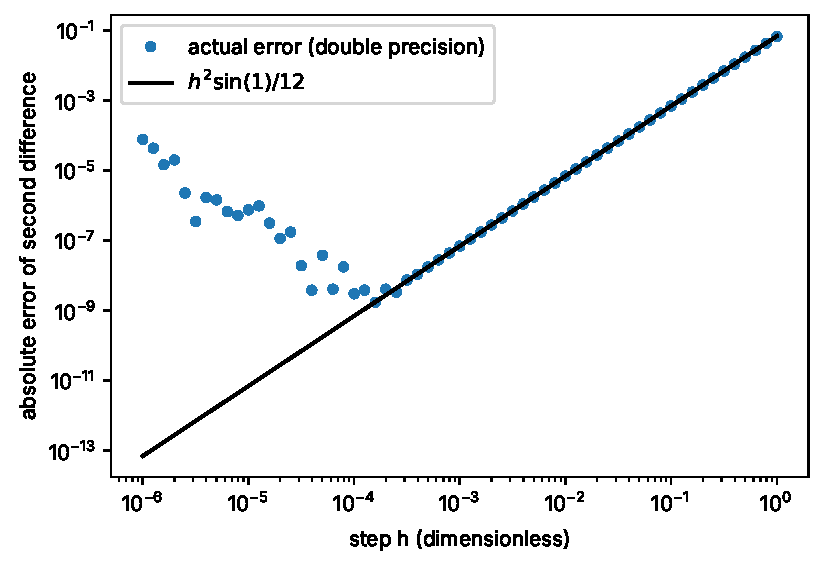
\includegraphics[width=0.85\linewidth]{figs/finite-differences_taylor.pdf}
\caption{Error of the central second difference $D_h^2\sin(1)$ as a function of the step $h$ (dimensionless). Dots: actual error computed in double precision. Line: the leading truncation error $h^2\sin(1)/12$ from Eq.~\eqref{eq:finite-differences-second-difference}. For $h$ above about $10^{-3}$ the dots follow the line of slope 2; for very small $h$ rounding error, of order $\epsilon/h^2$, takes over and the error grows again.}
\label{fig:finite-differences-taylor}
\end{figure}

\begin{checkpoint}
You compute a second derivative with $D_h^2$ and get an error of $8\times10^{-6}$. You repeat with $h$ divided by 10, still far from the roundoff regime. What error do you expect?
\end{checkpoint}
\checkanswer{About $8\times10^{-8}$: the error scales as $h^2$, so dividing $h$ by 10 divides the error by 100.}

\begin{pitfall}
Do not confuse ``second-order'' (error $\propto h^2$) with ``second derivative''. The forward difference \eqref{eq:finite-differences-forward} approximates a first derivative and is first-order; the central second difference approximates a second derivative and is second-order. The central \emph{first} difference $[f(x+h)-f(x-h)]/(2h)$ is also second-order (Problem~21).
\end{pitfall}

\begin{keyideas}
\item The central second difference $D_h^2f=[f(x+h)-2f(x)+f(x-h)]/h^2$ equals $f''+\tfrac{h^2}{12}f''''+\order(h^4)$, Eq.~\eqref{eq:finite-differences-second-difference}.
\item Its error contains only even powers of $h$ and is controlled by the fourth derivative: rapidly wiggling functions are hardest.
\item Rounding error grows like $\epsilon/h^2$, so very small steps eventually make things worse.
\end{keyideas}

%==========================================================
\section{The grid, the walls and the matrix}\label{sec:finite-differences-grid}

\subsection{Placing the points}

We want the levels of $H=-\dd^2/\dd x^2+V(x)$ in a box $[-L,L]$ with infinitely high walls at $x=\pm L$ (units $\hbar=2m=1$, as in Chapter~\ref{ch:schrodinger}). Recall from Chapter~\ref{ch:bound-states} that infinite walls force the wavefunction to vanish there: $\psi(-L)=\psi(L)=0$. A condition that fixes the value of the unknown function on the boundary is called a \emph{Dirichlet} boundary condition, so these are ``Dirichlet walls''.

Divide $[-L,L]$ into $N+1$ equal intervals. That creates $N+2$ points,
\begin{equation}
x_j=-L+jh,\qquad j=0,1,\dots,N+1,\qquad h=\frac{2L}{N+1}.
\label{eq:finite-differences-grid}
\end{equation}
The spacing formula follows because $N+1$ intervals of width $h$ must fill the length $2L$. The two end points $x_0=-L$ and $x_{N+1}=L$ sit on the walls. The other $N$ points, $x_1,\dots,x_N$, are the \emph{interior points}; for grids, the paper and \texttt{qmnt} use ``$N$'' for the number of interior points. Do not confuse it with the counting functions $N(T)$, $\Nsm$ and $\Nfl$, which the paper writes with the same letter. Write $\psi_j$ for our approximation to $\psi(x_j)$ and $V_j=V(x_j)$. The walls give
\begin{equation}
\psi_0=0,\qquad \psi_{N+1}=0,
\label{eq:finite-differences-walls}
\end{equation}
so only the $N$ interior values are unknown.

\subsection{One equation per interior point}

At each interior point $x_j$, replace $\psi''(x_j)$ in $-\psi''+V\psi=E\psi$ by the second difference \eqref{eq:finite-differences-second-difference} with step $h$, dropping the error terms:
\begin{equation}
-\frac{\psi_{j+1}-2\psi_j+\psi_{j-1}}{h^2}+V_j\psi_j=E\psi_j,\qquad j=1,\dots,N.
\label{eq:finite-differences-discrete-eq}
\end{equation}
Expand the left side to collect the coefficient of each unknown:
\begin{equation}
-\frac{1}{h^2}\psi_{j-1}+\left(\frac{2}{h^2}+V_j\right)\psi_j-\frac{1}{h^2}\psi_{j+1}=E\psi_j.
\label{eq:finite-differences-row}
\end{equation}
Now look at the two ends. For $j=1$ the equation involves $\psi_0$, which is zero by \eqref{eq:finite-differences-walls}, so that term disappears:
\begin{equation*}
\left(\frac{2}{h^2}+V_1\right)\psi_1-\frac{1}{h^2}\psi_2=E\psi_1.
\end{equation*}
For $j=N$ the term in $\psi_{N+1}$ disappears in the same way:
\begin{equation*}
-\frac{1}{h^2}\psi_{N-1}+\left(\frac{2}{h^2}+V_N\right)\psi_N=E\psi_N.
\end{equation*}

\subsection{The matrix form}

Collect the unknowns into a column vector $\bm\psi=(\psi_1,\dots,\psi_N)^\top$ (Chapter~\ref{ch:linear-algebra}). The $N$ equations \eqref{eq:finite-differences-row}, with the two end versions, say exactly $\mathsf H\bm\psi=E\bm\psi$, where $\mathsf H$ is the $N\times N$ matrix
\begin{equation}
\mathsf H=\begin{pmatrix}
\frac{2}{h^2}+V_1 & -\frac{1}{h^2} & 0 & \cdots & 0\\[2pt]
-\frac{1}{h^2} & \frac{2}{h^2}+V_2 & -\frac{1}{h^2} & \cdots & 0\\[2pt]
0 & -\frac{1}{h^2} & \frac{2}{h^2}+V_3 & \ddots & \vdots\\
\vdots & \vdots & \ddots & \ddots & -\frac{1}{h^2}\\[2pt]
0 & 0 & \cdots & -\frac{1}{h^2} & \frac{2}{h^2}+V_N
\end{pmatrix}.
\label{eq:finite-differences-matrix}
\end{equation}
Row $j$ of $\mathsf H$ holds the three coefficients of \eqref{eq:finite-differences-row}: $-1/h^2$ in column $j-1$, $2/h^2+V_j$ on the diagonal, and $-1/h^2$ in column $j+1$. The first and last rows have only two entries because the would-be third neighbor is a wall value that vanished.

Three properties follow at once from the pattern of entries.
\begin{enumerate}
\item $\mathsf H$ is \emph{tridiagonal}: nonzero only on the main diagonal and the two adjacent diagonals (Chapter~\ref{ch:eigen}). It has $N$ diagonal entries and $N-1$ entries on each of the two off-diagonals, so $N+2(N-1)=3N-2$ nonzero numbers.
\item $\mathsf H$ is \emph{real symmetric}: the entry in row $j$, column $j+1$ is $-1/h^2$, and so is the entry in row $j+1$, column $j$. By the theorem of Chapter~\ref{ch:eigen}, its eigenvalues are real and it has $N$ orthonormal eigenvectors. This is the discrete counterpart of $H$ being Hermitian (Chapter~\ref{ch:schrodinger}).
\item The continuous problem has infinitely many levels; the matrix has exactly $N$. Only the lowest ones, whose wavefunctions vary slowly on the scale of $h$, approximate physical levels. We will see in \cref{sec:finite-differences-box} how fast the approximation deteriorates.
\end{enumerate}

\begin{figure}[htbp]\centering
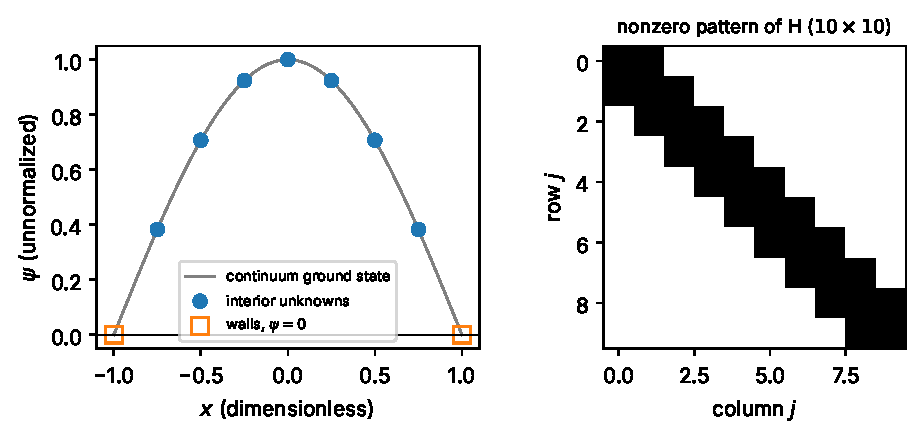
\includegraphics[width=0.85\linewidth]{figs/finite-differences_grid.pdf}
\caption{Left: the grid of Eq.~\eqref{eq:finite-differences-grid} for $N=7$ interior points on $[-1,1]$ (units $\hbar=2m=1$, $x$ dimensionless). Hollow squares: wall points where $\psi=0$; filled dots: the $N$ unknowns, here the sampled ground state of the box. Right: the pattern of the $7\times7$ matrix $\mathsf H$ of Eq.~\eqref{eq:finite-differences-matrix} with $V=0$; only three diagonals are nonzero.}
\label{fig:finite-differences-grid}
\end{figure}

\begin{sample}{A three-point box}
Take the box $[-1,1]$ ($L=1$) with $V=0$ and $N=3$ interior points. Build $\mathsf H$, find its eigenvalues from the characteristic polynomial, and compare them with the exact levels $E_k=(k\pi/2L)^2$ of Chapter~\ref{ch:bound-states}.

\textbf{Step 1: Spacing and points.} By \eqref{eq:finite-differences-grid}, $h=2L/(N+1)=2/4=0.5$, and the interior points are $x_1=-0.5$, $x_2=0$, $x_3=0.5$.

\textbf{Step 2: The matrix.} $2/h^2=2/0.25=8$ and $1/h^2=4$, so
\begin{equation*}
\mathsf H=\begin{pmatrix}8&-4&0\\-4&8&-4\\0&-4&8\end{pmatrix}.
\end{equation*}

\textbf{Step 3: Characteristic polynomial.} Write $a=8-\lambda$. Expanding $\det(\mathsf H-\lambda I)$ along the first row (Chapter~\ref{ch:linear-algebra}),
\begin{align*}
\det\begin{pmatrix}a&-4&0\\-4&a&-4\\0&-4&a\end{pmatrix}
&=a\,(a^2-16)-(-4)\big((-4)a-(-4)(0)\big)+0\\
&=a^3-16a-16a\\
&=a\,(a^2-32).
\end{align*}

\textbf{Step 4: Roots.} $a=0$ gives $\lambda=8$; $a^2=32$ gives $\lambda=8\pm\sqrt{32}=8\pm5.65685$. In increasing order the eigenvalues are $2.34315$, $8$, $13.65685$.

\textbf{Step 5: Compare.} The exact levels are $(\pi/2)^2=2.46740$, $\pi^2=9.86960$ and $(3\pi/2)^2=22.20661$. The relative errors are
\begin{equation*}
\boxed{\frac{2.46740-2.34315}{2.46740}=5.04\%,\quad \frac{9.86960-8}{9.86960}=18.9\%,\quad \frac{22.20661-13.65685}{22.20661}=38.5\%.}
\end{equation*}
Every computed level is too low, and the error grows rapidly with the level index. Three points per box is far too few; the next sections explain the pattern and how to beat it.
\end{sample}

\begin{checkpoint}
Why does the first row of $\mathsf H$ contain only two nonzero entries, while a middle row contains three?
\end{checkpoint}
\checkanswer{Row $j$ couples $\psi_j$ to its neighbors $\psi_{j-1}$ and $\psi_{j+1}$. For $j=1$ the left neighbor is the wall value $\psi_0$, which is zero by the Dirichlet condition, so its coefficient never enters the matrix.}

\subsection{Code}

The matrix is never stored as an $N\times N$ array; we hand the solver its two diagonals. Chapter~\ref{ch:eigen} introduced \texttt{scipy.linalg.eigh\_tridiagonal}, which calls the LAPACK routines for symmetric tridiagonal matrices and can return only the eigenvalues with indices in a requested range.

\begin{pycode}
import numpy as np
from scipy.linalg import eigh_tridiagonal

def fd_levels(V, L, k):
    """Lowest k levels of -d2/dx2 + V on (-L, L) with Dirichlet walls.
    V holds the potential at the N interior points."""
    N = len(V)
    h = 2 * L / (N + 1)                  # Eq. (grid)
    diag = 2.0 / h**2 + V                # main diagonal
    off = -np.ones(N - 1) / h**2         # the two off-diagonals
    return eigh_tridiagonal(diag, off, eigvals_only=True,
                            select='i', select_range=(0, k - 1))

print(fd_levels(np.zeros(3), 1.0, 3))    # 2.34315, 8, 13.65685
\end{pycode}

The library \texttt{qmnt} provides the same thing as \texttt{qmnt.fd\_levels(Vvals, L, k)}, together with \texttt{qmnt.grid(L, N)} for the interior points. In what follows we use whichever is more convenient.

\begin{keyideas}
\item With $h=2L/(N+1)$ and $\psi_0=\psi_{N+1}=0$, the equation $-\psi''+V\psi=E\psi$ becomes the $N\times N$ eigenproblem $\mathsf H\bm\psi=E\bm\psi$.
\item $\mathsf H$ is real symmetric tridiagonal: diagonal $2/h^2+V_j$, off-diagonals $-1/h^2$, Eq.~\eqref{eq:finite-differences-matrix}.
\item The matrix has only $N$ eigenvalues; only the low ones approximate physical levels.
\end{keyideas}

%==========================================================
\section{A test we can solve exactly: the box on a grid}\label{sec:finite-differences-box}
% DYK-BEGIN

% DYK-END

Before trusting a numerical method on a hard problem, test it on a problem whose answer you know. The infinite well with $V=0$ is perfect, because, remarkably, the \emph{discrete} problem can also be solved exactly. That will tell us precisely how the error depends on $h$ and on the level index.

\subsection{Exact eigenvectors of the discrete box}

With $V=0$, \eqref{eq:finite-differences-discrete-eq} reads
\begin{equation}
-\frac{\psi_{j+1}-2\psi_j+\psi_{j-1}}{h^2}=E\psi_j,\qquad \psi_0=\psi_{N+1}=0.
\label{eq:finite-differences-box-discrete}
\end{equation}
The continuum box has sine solutions, so try $\psi_j=\sin(j\theta)$ for some number $\theta$ to be found.

\textbf{The interior equation.} Use $\sin(a+b)+\sin(a-b)=2\sin a\cos b$ with $a=j\theta$, $b=\theta$:
\begin{equation*}
\psi_{j+1}+\psi_{j-1}=\sin((j+1)\theta)+\sin((j-1)\theta)=2\sin(j\theta)\cos\theta.
\end{equation*}
Subtract $2\psi_j=2\sin(j\theta)$:
\begin{equation*}
\psi_{j+1}-2\psi_j+\psi_{j-1}=2\sin(j\theta)\cos\theta-2\sin(j\theta)=-2(1-\cos\theta)\sin(j\theta).
\end{equation*}
Divide by $-h^2$:
\begin{equation*}
-\frac{\psi_{j+1}-2\psi_j+\psi_{j-1}}{h^2}=\frac{2(1-\cos\theta)}{h^2}\,\psi_j.
\end{equation*}
So $\sin(j\theta)$ satisfies \eqref{eq:finite-differences-box-discrete} at every interior point with $E=2(1-\cos\theta)/h^2$, \emph{whatever} $\theta$ is.

\textbf{The walls.} At $j=0$, $\psi_0=\sin0=0$ automatically. At $j=N+1$ we need $\sin((N+1)\theta)=0$, so $(N+1)\theta$ must be a whole multiple of $\pi$:
\begin{equation*}
\theta=\frac{k\pi}{N+1},\qquad k=1,2,\dots,N.
\end{equation*}

\textbf{The eigenvalues.} Using $1-\cos\theta=2\sin^2(\theta/2)$,
\begin{equation*}
E=\frac{2}{h^2}\cdot2\sin^2\frac{\theta}{2}=\frac{4}{h^2}\sin^2\frac{k\pi}{2(N+1)}.
\end{equation*}
Finally, $N+1=2L/h$ from \eqref{eq:finite-differences-grid}, so $\frac{k\pi}{2(N+1)}=\frac{k\pi h}{4L}$ and
\begin{equation}
\boxed{\;E_k^{(h)}=\frac{4}{h^2}\sin^2\!\left(\frac{k\pi h}{4L}\right),\qquad k=1,\dots,N.\;}
\label{eq:finite-differences-box-exact}
\end{equation}

\textbf{Have we found them all?} For $k=1,\dots,N$, the angle $k\pi/(2(N+1))$ lies strictly between $0$ and $\pi/2$, where $\sin^2$ is strictly increasing, so the $N$ values in \eqref{eq:finite-differences-box-exact} are distinct. An $N\times N$ matrix has exactly $N$ eigenvalues counted with multiplicity (Chapter~\ref{ch:eigen}), so these are all of them. (Problem~6 shows that $k=N+1$ gives the zero vector and that larger $k$ only repeat the same vectors.) Check with Sample Problem ``A three-point box'': $h=0.5$, $L=1$, $k=1$ gives $16\sin^2(\pi/8)=2.34315$, as found there.

\textbf{The eigenvectors are exact samples.} Since $j=(x_j+L)/h$ and $(N+1)h=2L$,
\begin{equation*}
j\theta=\frac{jk\pi}{N+1}=\frac{k\pi(x_j+L)}{2L}.
\end{equation*}
So the discrete eigenvector is $\psi_j=\sin\big(k\pi(x_j+L)/(2L)\big)$: precisely the continuum eigenfunction of Chapter~\ref{ch:bound-states}, sampled at the grid points. For the box, the grid gets the \emph{shape} of every state exactly right and only the \emph{energy} wrong. That is special to $V=0$, but it is a very clean laboratory.

\subsection{How wrong is the energy?}

Compare \eqref{eq:finite-differences-box-exact} with the exact level $E_k=(k\pi/2L)^2$. Introduce $y=k\pi h/(4L)$. Then
\begin{equation*}
\frac{4}{h^2}y^2=\frac{4}{h^2}\frac{k^2\pi^2h^2}{16L^2}=\left(\frac{k\pi}{2L}\right)^2=E_k,
\end{equation*}
so $E_k=(4/h^2)y^2$ and $E_k^{(h)}=(4/h^2)\sin^2y$. Expand $\sin^2y$ using $\sin^2y=(1-\cos2y)/2$ and the cosine series $\cos u=1-u^2/2+u^4/24-u^6/720+\cdots$ with $u=2y$:
\begin{align*}
\sin^2y&=\frac12\left[\frac{(2y)^2}{2}-\frac{(2y)^4}{24}+\frac{(2y)^6}{720}-\cdots\right]\\
&=\frac{4y^2}{4}-\frac{16y^4}{48}+\frac{64y^6}{1440}-\cdots\\
&=y^2-\frac{y^4}{3}+\frac{2y^6}{45}-\cdots.
\end{align*}
Multiply by $4/h^2$:
\begin{equation*}
E_k^{(h)}=\frac{4}{h^2}y^2-\frac{4}{3h^2}y^4+\frac{8}{45h^2}y^6-\cdots.
\end{equation*}
Express each power of $y$ through $E_k$, using $y^2=h^2E_k/4$, so $y^4=h^4E_k^2/16$ and $y^6=h^6E_k^3/64$:
\begin{align*}
\frac{4}{3h^2}y^4&=\frac{4}{3h^2}\cdot\frac{h^4E_k^2}{16}=\frac{h^2E_k^2}{12},\\
\frac{8}{45h^2}y^6&=\frac{8}{45h^2}\cdot\frac{h^6E_k^3}{64}=\frac{h^4E_k^3}{360}.
\end{align*}
Therefore
\begin{equation}
\boxed{\;E_k^{(h)}=E_k-\frac{h^2}{12}E_k^2+\frac{h^4}{360}E_k^3-\cdots\;}
\label{eq:finite-differences-box-expansion}
\end{equation}
Three lessons are packed into this formula.
\begin{itemize}
\item The grid levels are \emph{below} the true levels for every $k$: exactly so, because $\sin^2y<y^2$ for every $y>0$ in Eq.~\eqref{eq:finite-differences-box-exact}; the series gives the leading size of the deficit.
\item The error is $\order(h^2)$, as \eqref{eq:finite-differences-second-difference} promised, with only even powers of $h$.
\item At fixed $h$ the error grows like $E_k^2$, that is like $k^4$. The relative error, $h^2E_k/12$, grows like $k^2$. High levels are far worse than low ones.
\end{itemize}
The expansion is useful only when $y=k\pi h/(4L)$ is small, that is when the level index $k$ is small compared with the number of points $N$. When $k$ approaches $N$ the exact formula \eqref{eq:finite-differences-box-exact} must be used.

\subsection{The same thing in the language of waves: numerical dispersion}

There is a more physical way to see \eqref{eq:finite-differences-box-exact}. Feed the complex wave $e^{iqx}$ (Chapter~\ref{ch:complex}) into the second difference:
\begin{align*}
D_h^2e^{iqx}&=\frac{e^{iq(x+h)}-2e^{iqx}+e^{iq(x-h)}}{h^2}\\
&=e^{iqx}\,\frac{e^{iqh}+e^{-iqh}-2}{h^2}\\
&=e^{iqx}\,\frac{2\cos(qh)-2}{h^2}\qquad\text{(since }e^{i\theta}+e^{-i\theta}=2\cos\theta\text{)}\\
&=-\frac{4}{h^2}\sin^2\!\left(\frac{qh}{2}\right)e^{iqx}\qquad\text{(since }1-\cos\theta=2\sin^2(\theta/2)\text{)}.
\end{align*}
The exact operator $-\dd^2/\dd x^2$ multiplies $e^{iqx}$ by $q^2$: a free particle of wavenumber $q$ has kinetic energy $q^2$ in our units. The grid operator multiplies it instead by
\begin{equation}
K_h(q)=\frac{4}{h^2}\sin^2\!\left(\frac{qh}{2}\right).
\label{eq:finite-differences-dispersion}
\end{equation}
A box state is a standing wave with $q_k=k\pi/(2L)$ (Chapter~\ref{ch:bound-states}), and indeed $K_h(q_k)$ is exactly \eqref{eq:finite-differences-box-exact}. A rule relating energy (or frequency) to wavenumber is called a \emph{dispersion relation}, so the error is often called \emph{numerical dispersion}: the grid gets the kinetic energy of long waves right and systematically underestimates it for short waves.

The natural measure of ``short'' is the number of grid points per wavelength, $n_{\rm pw}=\lambda/h=2\pi/(qh)$. Then $qh/2=\pi/n_{\rm pw}$ and
\begin{equation}
\frac{K_h(q)}{q^2}=\left[\frac{\sin(\pi/n_{\rm pw})}{\pi/n_{\rm pw}}\right]^2.
\label{eq:finite-differences-ppw}
\end{equation}
\Cref{tab:finite-differences-ppw} evaluates the relative error $1-K_h/q^2$. The shortest wave a grid can carry alternates sign from point to point, $n_{\rm pw}=2$, $qh=\pi$; there $K_h=4/h^2$, the largest value \eqref{eq:finite-differences-dispersion} can take.

\begin{table}[htbp]\centering
\caption{Relative underestimate $1-K_h(q)/q^2$ of the kinetic energy of a wave sampled with $n_{\rm pw}$ grid points per wavelength, Eq.~\eqref{eq:finite-differences-ppw}.}
\label{tab:finite-differences-ppw}
\begin{tabular}{ccccccc}
\toprule
$n_{\rm pw}$ & 4 & 6 & 8 & 12 & 24 & 50\\
\midrule
$1-K_h/q^2$ & 18.9\% & 8.81\% & 5.04\% & 2.26\% & 0.570\% & 0.13\%\\
\bottomrule
\end{tabular}
\end{table}

The $n_{\rm pw}=4$ entry reproduces the middle level of the three-point box: there $k=2$, $q=\pi$, $h=0.5$, so $qh=\pi/2$ and four points per wavelength, error $18.9\%$.

\begin{figure}[htbp]\centering
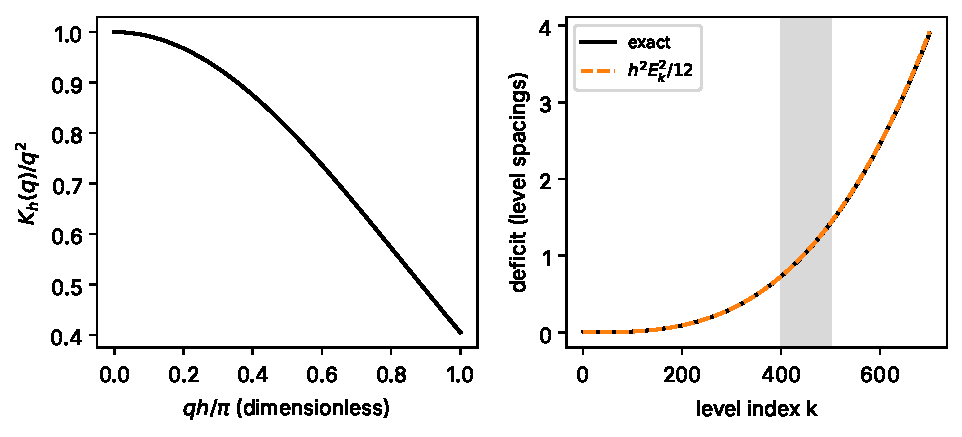
\includegraphics[width=0.85\linewidth]{figs/finite-differences_dispersion.pdf}
\caption{Left: the grid dispersion relation $K_h(q)/q^2$ of Eq.~\eqref{eq:finite-differences-dispersion} against $qh/\pi$ (both dimensionless); the right end, $qh=\pi$, is the zigzag wave with two points per wavelength. Right: the box of running example RE3, $L=44.883$, $N=6000$ (units $\hbar=2m=1$): the deficit $E_k-E_k^{(h)}$ in units of the local box level spacing $E_{k+1}-E_k$, exact (solid) and leading-order estimate $h^2E_k^2/12$ (dashed). The shaded band marks $k=401$--$500$.}
\label{fig:finite-differences-dispersion}
\end{figure}

\begin{sample}{The paper's grid applied to the empty box (RE3)}
Running example RE3 is the box $[-L,L]$ with $L=44.883$, the half-width the paper uses at scale 1. Put $N=6000$ interior points in it, the paper's working grid at scale 1, with $V=0$. Find the error in level $k=500$ in energy units and in units of the local level spacing of the box, and the number of grid points per wavelength.

\textbf{Step 1: Spacing.} $h=2L/(N+1)=89.766/6001=0.0149585$, so $h^2=2.23757\times10^{-4}$ and $4/h^2=17876.5$.

\textbf{Step 2: Exact level.} $E_{500}=(500\pi/89.766)^2=306.21$.

\textbf{Step 3: Grid level.} The argument in \eqref{eq:finite-differences-box-exact} is $k\pi h/(4L)=500\pi/12002=0.130878$, and $\sin^2(0.130878)=0.0170314$, so $E^{(h)}_{500}=17876.5\times0.0170314=304.46$.

\textbf{Step 4: Error.} $E_{500}-E^{(h)}_{500}=1.744$. The leading term of \eqref{eq:finite-differences-box-expansion}, $h^2E_{500}^2/12=1.748$, agrees to better than half a percent; the relative error is $0.570\%$.

\textbf{Step 5: In units of the level spacing.} Box levels are spaced by $E_{k+1}-E_k=(2k+1)(\pi/2L)^2$, which for $k=500$ is $1001\times1.22483\times10^{-3}=1.226$. So
\begin{equation*}
\boxed{E_{500}-E^{(h)}_{500}=1.74\ \text{energy units}=1.42\ \text{level spacings}.}
\end{equation*}

\textbf{Step 6: Points per wavelength.} With $q=500\pi/(2L)$, $n_{\rm pw}=2\pi/(qh)=4L/(500h)=2(N+1)/500=24.0$. \Cref{tab:finite-differences-ppw} says $24$ points per wavelength costs $0.570\%$, matching Step 4.

By contrast the ground state, $E_1=1.22483\times10^{-3}$, has error $h^2E_1^2/12\approx3\times10^{-11}$, completely negligible. A grid that is superb for low levels can misplace level 500 by more than a level spacing.
\end{sample}

\begin{checkpoint}
On a uniform grid, is the computed ground-state energy of the infinite well above or below the exact value? Does the answer change for level 500?
\end{checkpoint}
\checkanswer{Below, for every level: $\sin^2y<y^2$ for $0<y\le\pi/2$, so $E_k^{(h)}<E_k$ by Eq.~\eqref{eq:finite-differences-box-exact}. The deficit is just much larger for level 500.}

\begin{keyideas}
\item The discrete box is exactly solvable: eigenvectors are sampled sines and $E_k^{(h)}=(4/h^2)\sin^2(k\pi h/4L)$, Eq.~\eqref{eq:finite-differences-box-exact}.
\item $E_k^{(h)}=E_k-h^2E_k^2/12+h^4E_k^3/360-\cdots$: always too low, error growing like $E_k^2$.
\item In wave language, the grid replaces $q^2$ by $(4/h^2)\sin^2(qh/2)$ (numerical dispersion); accuracy is set by points per wavelength.
\item On the paper's scale-1 grid, box level 500 is off by about $1.4$ level spacings.
\end{keyideas}

%==========================================================
\section{General potentials: estimating the grid bias}\label{sec:finite-differences-bias}

For the box we had an exact formula. For a general potential we need an estimate. The idea is simple: the grid operator is the true operator plus a small extra piece, and a small extra piece in a matrix shifts each eigenvalue by its ``expectation value''. Chapter~\ref{ch:perturbation} develops this idea, perturbation theory, at length; here we need only its first step, and we prove it directly for matrices.

\subsection{How an eigenvalue moves when a symmetric matrix changes}

Let $\mathsf H(\varepsilon)=\mathsf H_0+\varepsilon\mathsf W$, where $\mathsf H_0$ and $\mathsf W$ are real symmetric $N\times N$ matrices and $\varepsilon$ is a real number. Suppose $E(\varepsilon)$ is an eigenvalue that stays distinct from all the others as $\varepsilon$ varies, with a unit eigenvector $\mathbf u(\varepsilon)$, so that
\begin{equation*}
\mathsf H(\varepsilon)\mathbf u(\varepsilon)=E(\varepsilon)\mathbf u(\varepsilon),\qquad \mathbf u^\top\mathbf u=1.
\end{equation*}

\begin{beyond}
That a non-repeated eigenvalue and its eigenvector depend smoothly (differentiably) on $\varepsilon$ is a standard theorem of matrix perturbation theory, which we take on trust. Its proof applies the implicit function theorem to the characteristic equation $\det(\mathsf H(\varepsilon)-E\,I)=0$ at a simple root (where the derivative of the determinant with respect to $E$ is nonzero), and then to the linear equations for the eigenvector; it is found in standard texts on matrix perturbation theory. Everything below is then ordinary calculus.
\end{beyond}

Differentiate the eigen-equation with respect to $\varepsilon$, using the product rule and writing a prime for $\dd/\dd\varepsilon$:
\begin{equation*}
\mathsf W\mathbf u+\mathsf H\mathbf u'=E'\mathbf u+E\mathbf u'.
\end{equation*}
Multiply on the left by the row vector $\mathbf u^\top$:
\begin{equation*}
\mathbf u^\top\mathsf W\mathbf u+\mathbf u^\top\mathsf H\mathbf u'=E'\,\mathbf u^\top\mathbf u+E\,\mathbf u^\top\mathbf u'.
\end{equation*}
Because $\mathsf H$ is symmetric, $\mathbf u^\top\mathsf H=(\mathsf H\mathbf u)^\top=E\mathbf u^\top$, so the second term on the left is $E\,\mathbf u^\top\mathbf u'$, which cancels the last term on the right. With $\mathbf u^\top\mathbf u=1$ what remains is
\begin{equation}
\boxed{\;\frac{\dd E}{\dd\varepsilon}=\mathbf u^\top\mathsf W\mathbf u=\sum_{i,j}u_iW_{ij}u_j.\;}
\label{eq:finite-differences-hf}
\end{equation}
For a small change $\varepsilon\mathsf W$, the eigenvalue moves by approximately $\varepsilon\,\mathbf u^\top\mathsf W\mathbf u$. The continuum version, which Chapter~\ref{ch:perturbation} derives, reads $\delta E\approx\int\psi\,\delta H\,\psi\,\dd x$. Keep \eqref{eq:finite-differences-hf} in mind: we will use it twice more in this chapter.

\begin{sample}{An eigenvalue nudged by hand}
Take the three-point box of Sample Problem ``A three-point box'' ($L=1$, $h=0.5$, $V=0$) and add $\varepsilon$ to the middle diagonal entry only, so $\mathsf W=\mathrm{diag}(0,1,0)$. Predict $\dd E/\dd\varepsilon$ for the lowest eigenvalue from Eq.~\eqref{eq:finite-differences-hf} and test the prediction at $\varepsilon=0.01$.

\textbf{Step 1: The unit eigenvector.} By \cref{sec:finite-differences-box}, the lowest eigenvector is proportional to $(\sin\frac\pi4,\sin\frac\pi2,\sin\frac{3\pi}4)=(0.7071,1,0.7071)$. Its squares sum to $0.5+1+0.5=2$, so dividing by $\sqrt2$ gives the unit vector $\mathbf u=(0.5,0.7071,0.5)$.

\textbf{Step 2: Predict.} $\mathbf u^\top\mathsf W\mathbf u=u_2^2=0.5$, so the lowest eigenvalue should rise by about $0.5\varepsilon=5.000\times10^{-3}$, from $2.343146$ to $2.348146$.

\textbf{Step 3: Exact.} The lowest eigenvalue of the matrix with rows $(8,-4,0)$, $(-4,8.01,-4)$, $(0,-4,8)$, computed with \texttt{np.linalg.eigvalsh}, is $2.3481435$, a rise of $4.998\times10^{-3}$.
\begin{equation*}
\boxed{\frac{\dd E}{\dd\varepsilon}=0.5;\quad\text{predicted shift }5.000\times10^{-3},\ \text{exact }4.998\times10^{-3}.}
\end{equation*}
The tiny difference is the next term of the expansion in $\varepsilon$, of order $\varepsilon^2$.
\end{sample}

\subsection{The grid as a perturbed Hamiltonian}

By \eqref{eq:finite-differences-second-difference}, applied to a smooth wavefunction, $-D_h^2\psi=-\psi''-\tfrac{h^2}{12}\psi''''-\cdots$. So, acting on smooth functions, the grid Hamiltonian looks like the true Hamiltonian plus an extra operator,
\begin{equation*}
H_{\rm grid}\approx H+W,\qquad W=-\frac{h^2}{12}\frac{\dd^4}{\dd x^4}.
\end{equation*}
This step is heuristic, for three reasons: Eq.~\eqref{eq:finite-differences-hf} was proved for matrices, not for differential operators; the replacement of the grid operator by $H+W$ holds only when acting on smooth functions; and $W$ is not a small operator in general (it is large on rapidly varying functions). We nevertheless treat $W$ as a small perturbation and carry Eq.~\eqref{eq:finite-differences-hf} over to functions. If $\psi$ is normalized, $\int\psi^2\,\dd x=1$, then the grid vector with entries $u_j=\sqrt h\,\psi(x_j)$ is approximately a unit vector, because $\sum_ju_j^2=\sum_j\psi(x_j)^2h$ is a Riemann sum for $\int\psi^2\,\dd x$. Likewise $\mathbf u^\top\mathsf W\mathbf u=\sum_j\psi(x_j)\,(W\psi)(x_j)\,h$ is a Riemann sum for $\int\psi\,W\psi\,\dd x$. So the continuum form of Eq.~\eqref{eq:finite-differences-hf} is $\delta E\approx\int\psi\,\delta H\,\psi\,\dd x$ (Chapter~\ref{ch:perturbation} reaches the same formula directly in the continuum). Then the grid level should sit at
\begin{equation*}
E_n^{\rm grid}-E_n\approx\int_{-L}^{L}\psi_n\,W\psi_n\,\dd x=-\frac{h^2}{12}\int_{-L}^{L}\psi_n\,\psi_n''''\,\dd x,
\end{equation*}
where $\psi_n$ is the normalized true eigenfunction (real, as bound states in one dimension can be chosen, Chapter~\ref{ch:bound-states}). Integrate by parts twice:
\begin{align*}
\int_{-L}^{L}\psi_n\psi_n''''\,\dd x&=\Big[\psi_n\psi_n'''\Big]_{-L}^{L}-\int_{-L}^{L}\psi_n'\psi_n'''\,\dd x\\
&=\Big[\psi_n\psi_n'''\Big]_{-L}^{L}-\Big[\psi_n'\psi_n''\Big]_{-L}^{L}+\int_{-L}^{L}(\psi_n'')^2\,\dd x.
\end{align*}
At the walls $\psi_n=0$, so the first bracket vanishes. For the second, use the Schr\"odinger equation, $\psi_n''=(V-E_n)\psi_n$, which also vanishes at the walls, provided $V$ is finite and smooth up to the walls, so that $\psi_n''$ is continuous up to the wall (true for ours: the Wu--Sprung potential is smooth and only about $1000$ at $x=\pm L$). So both brackets are zero and
\begin{equation*}
\int\psi_n\psi_n''''\,\dd x=\int(\psi_n'')^2\,\dd x=\int(E_n-V)^2\psi_n^2\,\dd x.
\end{equation*}
Therefore
\begin{equation}
\boxed{\;E_n^{\rm grid}-E_n\approx-\frac{h^2}{12}\int_{-L}^{L}\big(E_n-V(x)\big)^2\psi_n(x)^2\,\dd x\equiv-\frac{h^2}{12}\big\langle(E_n-V)^2\big\rangle_n.\;}
\label{eq:finite-differences-bias-estimate}
\end{equation}

\begin{pitfall}
Equation \eqref{eq:finite-differences-bias-estimate} is a \textbf{heuristic, leading-order estimate}, not a theorem. The operator $\dd^4/\dd x^4$ is not small for rapidly varying functions, so the estimate is trustworthy only when the wavelength of the state is long compared with $h$ (many points per wavelength everywhere the state lives). It neglects the $h^4$ terms and the change of the wavefunction caused by the grid. For the box it reproduces the exact leading term of \eqref{eq:finite-differences-box-expansion}: with $V=0$, $\langle(E_n-0)^2\rangle=E_n^2$.
\end{pitfall}

\subsection{What the estimate says}

The quantity $E_n-V(x)$ is the local kinetic energy, and in our units it equals the square of the local wavenumber, $q(x)^2=E_n-V(x)$, inside the classically allowed region. So \eqref{eq:finite-differences-bias-estimate} says: the grid bias of a level is $h^2/12$ times the average of $q(x)^4$ over the state. Where the particle moves fast (deep in the well, high above the potential) the wave is short and the grid underestimates it most. Near a classical turning point $q\to0$ and the grid does well. This is the general version of the box statement ``error grows like $E^2$''.

\begin{sample}{Grid bias for the harmonic oscillator}
Recall from Chapter~\ref{ch:bound-states} that in units $\hbar=2m=1$ the Hamiltonian $H=-\dd^2/\dd x^2+x^2$ has ground state $\psi_0\propto e^{-x^2/2}$ with $E_0=1$. (Oscillator states are traditionally numbered from $n=0$; do not confuse this $\psi_0$ with the wall value $\psi_0=0$ of Eq.~\eqref{eq:finite-differences-walls}.) Estimate the grid bias of $E_0$ for $h=0.1$ and predict the computed value.

\textbf{Step 1: The integrand.} $E_0-V=1-x^2$, so $(E_0-V)^2=1-2x^2+x^4$ and
\begin{equation*}
\langle(E_0-V)^2\rangle=1-2\langle x^2\rangle+\langle x^4\rangle.
\end{equation*}

\textbf{Step 2: The moments.} With $\psi_0^2=\pi^{-1/2}e^{-x^2}$ and the Gaussian integrals $\int e^{-x^2}\dd x=\sqrt\pi$, $\int x^2e^{-x^2}\dd x=\sqrt\pi/2$, $\int x^4e^{-x^2}\dd x=3\sqrt\pi/4$ (Problem~10 asks you to derive them by integration by parts), $\langle x^2\rangle=1/2$ and $\langle x^4\rangle=3/4$.

\textbf{Step 3: Combine.} $\langle(E_0-V)^2\rangle=1-1+\tfrac34=\tfrac34$, so by \eqref{eq:finite-differences-bias-estimate}
\begin{equation*}
E_0^{\rm grid}-E_0\approx-\frac{h^2}{12}\cdot\frac34=-\frac{h^2}{16}=-6.25\times10^{-4}.
\end{equation*}

\textbf{Step 4: Predict.} 
\begin{equation*}
\boxed{E_0^{\rm grid}\approx0.999375.}
\end{equation*}
Solving the tridiagonal problem on $[-10,10]$ with $N=199$ (so $h=20/200=0.1$; the walls are so far out that $\psi_0$ is negligible there) gives this value to within a few times $10^{-6}$, as Problem~12 lets you confirm. Notice that the box formula $h^2E_0^2/12=8.3\times10^{-4}$ would overestimate the bias: the potential slows the particle down, and the state spends time near its turning points.
\end{sample}

\subsection{Why levels 401--500 are hard}

Now we can see the size of the problem the paper faced. At scale~1 the paper uses $L=44.883$ and $N=6000$ interior points, the same $h=0.0149585$ as our box example. Its levels 401--500 lie at heights roughly between $t_{401}$ and $t_{500}=811.18$ (the latter from the paper's Appendix~A key anchors). Two things conspire:
\begin{itemize}
\item The bias \eqref{eq:finite-differences-bias-estimate} grows roughly like the square of the local kinetic energy, and these are high levels. At the bottom of the Wu--Sprung well, where $V=V_0=3.10073\pi$, a level at $E=811.18$ has $q=\sqrt{E-V_0}=28.31$ and therefore only $2\pi/(qh)=14.8$ points per wavelength. This is the \emph{shortest} local wavelength of the state, reached at the bottom of the well where the kinetic energy is largest; elsewhere the wave is longer and better resolved, so this is a worst case, not a typical value.
\item The quantity we care about is not the energy error but the error in units of the \emph{mean spacing of the zeros}, which near height $t$ is $2\pi/\log(t/2\pi)$ (Chapter~\ref{ch:counting-zeros} derives this) and is only about $1.3$ near $t=811$. The spacing shrinks while the bias grows.
\end{itemize}
The paper reports the result: the finite-difference dispersion ``at levels 401--500 on the working grid reaches two mean spacings'' (Sec.~II~C). The fluctuations of the zeros that the paper studies have an rms of only about $0.26$ mean spacings on this range (the null of $0.263$). A bias about eight times larger than the signal ($2/0.263\approx7.6$) cannot be left in.

\begin{checkpoint}
Two levels of the same potential are computed on the same grid: level 10 and level 400. Which is more accurate in energy units, and why?
\end{checkpoint}
\checkanswer{Level 10. The bias is $h^2/12$ times the average of $(E-V)^2$, the fourth power of the local wavenumber; level 400 has far more kinetic energy, hence far shorter waves and far fewer points per wavelength.}

\begin{keyideas}
\item For a symmetric matrix, a small change $\varepsilon\mathsf W$ moves a non-repeated eigenvalue by $\varepsilon\,\mathbf u^\top\mathsf W\mathbf u$, Eq.~\eqref{eq:finite-differences-hf}.
\item Heuristically, the grid bias of level $n$ is $-\tfrac{h^2}{12}\langle(E_n-V)^2\rangle$, Eq.~\eqref{eq:finite-differences-bias-estimate}: $h^2/12$ times the mean fourth power of the local wavenumber.
\item On the paper's working grid this bias reaches about two mean spacings at levels 401--500 (paper Sec.~II~C), far larger than the fluctuations being studied.
\end{keyideas}

%==========================================================
\section{Richardson extrapolation}\label{sec:finite-differences-richardson}

We could shrink the bias by brute force: more points. Because the error is $\order(h^2)$, cutting it by a factor of 100 costs ten times as many points. There is a much cheaper trick, named after the meteorologist Lewis Fry Richardson. It exploits the fact that we know \emph{how} the error depends on $h$, even though we do not know its size.

\subsection{The derivation}

For a given level, write its computed value on a grid of spacing $h$ as $E(h)$. For the box we proved, in Eq.~\eqref{eq:finite-differences-box-expansion}, that the error is a series in even powers of $h$. For a general potential, Eq.~\eqref{eq:finite-differences-second-difference} makes this plausible, since the local error of $D_h^2$ contains only even powers of $h$; but that equation describes the difference operator acting on a fixed function, not the eigenvalues of the grid matrix, so for a general smooth potential the eigenvalue expansion is an assumption here (see the box below). We assume
\begin{equation}
E(h)=E+Ch^2+Dh^4+\order(h^6),
\label{eq:finite-differences-error-series}
\end{equation}
where $E$ is the exact level and $C$, $D$ are numbers that depend on the level and the potential but not on $h$.

\begin{beyond}
For a smooth potential on a finite interval with Dirichlet walls, the eigenvalues of the second-order finite-difference matrix do have, for each fixed level, an expansion $E(h)=E+Ch^2+Dh^4+\cdots$ in even powers of $h$. We take this on trust. Its proof belongs to the numerical analysis of finite-difference eigenvalue problems and is found in advanced texts on that subject; in this book it is proved only for the box, Eq.~\eqref{eq:finite-differences-box-expansion}. You need not trust it blindly: condition 2 below gives an empirical test (successive differences should shrink by a factor close to 4), and Problem~25 applies it.
\end{beyond} Now compute the same level on a grid with half the spacing:
\begin{equation*}
E(h/2)=E+C\frac{h^2}{4}+D\frac{h^4}{16}+\order(h^6).
\end{equation*}
Multiply this by 4:
\begin{equation*}
4E(h/2)=4E+Ch^2+D\frac{h^4}{4}+\order(h^6).
\end{equation*}
Subtract \eqref{eq:finite-differences-error-series}; the $Ch^2$ terms cancel:
\begin{equation*}
4E(h/2)-E(h)=3E+D\left(\frac14-1\right)h^4+\order(h^6)=3E-\frac34Dh^4+\order(h^6).
\end{equation*}
Divide by 3:
\begin{equation}
\boxed{\;E^{\rm Rich}\equiv\frac{4E(h/2)-E(h)}{3}=E-\frac{D}{4}h^4+\order(h^6).\;}
\label{eq:finite-differences-richardson}
\end{equation}
The unknown $h^2$ error has been eliminated without ever knowing $C$. The combination \eqref{eq:finite-differences-richardson} is what \texttt{qmnt.richardson(E\_h, E\_h2)} returns. For the box, $D=E^3/360$ by \eqref{eq:finite-differences-box-expansion}, so the Richardson error is
\begin{equation}
E^{\rm Rich}-E\approx-\frac{h^4E^3}{1440}\qquad\text{(box, leading order)}.
\label{eq:finite-differences-rich-box}
\end{equation}

\textbf{Unequal refinement.} If the fine spacing is $h/r$ rather than $h/2$, repeat the argument: $E(h/r)=E+Ch^2/r^2+\cdots$, multiply by $r^2$ and subtract $E(h)$ to get $r^2E(h/r)-E(h)=(r^2-1)E+\order(h^4)$, so
\begin{equation}
E^{\rm Rich}=\frac{r^2E(h/r)-E(h)}{r^2-1}+\order(h^4).
\label{eq:finite-differences-richardson-r}
\end{equation}
With $r=2$ this is \eqref{eq:finite-differences-richardson}.

\subsection{Conditions for Richardson to work}

Every step above relied on something; here is the list.
\begin{enumerate}
\item \textbf{The same level on both grids.} $E(h)$ and $E(h/2)$ must be the \emph{same} physical level. The grid matrix has no repeated eigenvalues. Proof: suppose $\mathsf H\mathbf v=\lambda\mathbf v$. The first row of $\mathsf H$ gives $(2/h^2+V_1-\lambda)v_1-v_2/h^2=0$, which fixes $v_2$ once $v_1$ is known; row $j$, Eq.~\eqref{eq:finite-differences-row}, then fixes $v_{j+1}$ from $v_j$ and $v_{j-1}$, because the coefficient $-1/h^2$ of $v_{j+1}$ is not zero. So $v_1=0$ forces $\mathbf v=0$, and every eigenvector for $\lambda$ is a multiple of the one with $v_1=1$: each eigenspace is one-dimensional. For a symmetric matrix the number of times an eigenvalue is repeated equals the dimension of its eigenspace (spectral theorem, Chapter~\ref{ch:eigen}), so all $N$ eigenvalues are distinct. (The continuum counterpart is the non-degeneracy of one-dimensional bound states, Chapter~\ref{ch:bound-states}.) The solver returns them sorted, so ``the $n$-th smallest eigenvalue on each grid'' identifies the level, as long as $n$ is far below $N$.
\item \textbf{The asymptotic regime.} The expansion \eqref{eq:finite-differences-error-series} must be dominated by its first term, which requires many points per wavelength. A practical test: the ratio $[E(h)-E(h/2)]/[E(h/2)-E(h/4)]$ should be close to 4.
\item \textbf{Smoothness.} The derivation of \eqref{eq:finite-differences-second-difference} needs a smooth wavefunction, which needs a smooth potential. A kink in $V$ (for example $\abs{x}$ at $x=0$) makes $\psi''$ jump in slope there, so the Taylor argument fails at the kink, the clean even-power expansion is no longer guaranteed, and neither is Richardson's cancellation; the ratio test of condition 2 is the practical way to detect such trouble.
\item \textbf{The right weights.} The \emph{finer} grid gets the weight 4. Swapping them makes things worse, not better (Problem~31).
\item \textbf{Exact halving.} Halving $h$ means doubling $N+1$, not $N$. Doubling $N$ gives a ratio $r$ slightly below 2; \eqref{eq:finite-differences-richardson-r} shows how small the resulting mistake is (Problem~11).
\end{enumerate}

\begin{sample}{Richardson on the three-point box}
Using $L=1$, $V=0$, combine the ground-state energies on grids with $N=3$ ($h=0.5$) and $N=7$ ($h=0.25$) into a Richardson estimate, and compare all three errors with the exact $E_1=\pi^2/4=2.467401$.

\textbf{Step 1: Coarse grid.} From the three-point box Sample Problem, $E(0.5)=16\sin^2(\pi/8)=2.343146$.

\textbf{Step 2: Fine grid.} $N=7$ gives $h=2/8=0.25$, exactly half (because $N+1$ doubled from 4 to 8). Then $4/h^2=64$ and $k\pi h/(4L)=\pi/16$, so $E(0.25)=64\sin^2(\pi/16)=2.435855$.

\textbf{Step 3: Combine.} 
\begin{equation*}
E^{\rm Rich}=\frac{4(2.435855)-2.343146}{3}=\frac{9.743420-2.343146}{3}=2.466758.
\end{equation*}

\textbf{Step 4: Errors.} $E_1-E(0.5)=0.1243$; $E_1-E(0.25)=0.0315$; $E_1-E^{\rm Rich}=6.4\times10^{-4}$. The prediction \eqref{eq:finite-differences-rich-box} gives $h^4E_1^3/1440=(0.0625)(15.02)/1440=6.5\times10^{-4}$ for $h=0.5$. So
\begin{equation*}
\boxed{E^{\rm Rich}=2.46676,\ \text{error }6.4\times10^{-4},\ \text{about 50 times smaller than on the finer grid alone.}}
\end{equation*}
\end{sample}

\begin{pycode}
import numpy as np, qmnt
L = 1.0
E_h  = qmnt.fd_levels(np.zeros(3), L, k=1)    # h = 0.5
E_h2 = qmnt.fd_levels(np.zeros(7), L, k=1)    # h = 0.25, exactly half
E_R  = qmnt.richardson(E_h, E_h2)             # (4*E_h2 - E_h)/3
print(E_h, E_h2, E_R, np.pi**2 / 4)
\end{pycode}

\begin{figure}[htbp]\centering
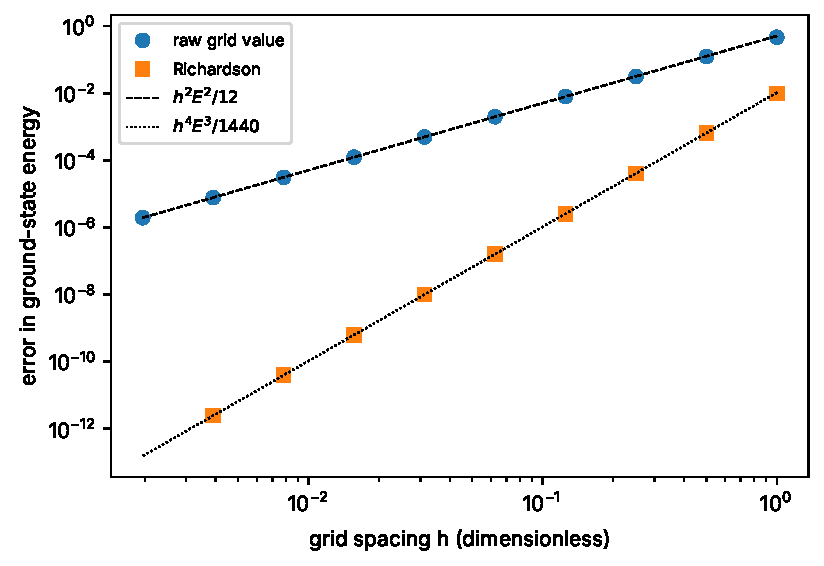
\includegraphics[width=0.85\linewidth]{figs/finite-differences_richardson.pdf}
\caption{Error in the ground-state energy of the box $[-1,1]$ (units $\hbar=2m=1$) against grid spacing $h$, with $N+1=2,4,8,\dots$ so that $h$ halves exactly. Circles: raw grid value, Eq.~\eqref{eq:finite-differences-box-exact}, slope 2. Squares: Richardson combination of each grid with the next finer one, Eq.~\eqref{eq:finite-differences-richardson}, slope 4. Dashed lines: the leading-order predictions $h^2E^2/12$ and $h^4E^3/1440$.}
\label{fig:finite-differences-richardson}
\end{figure}

\begin{sample}{Brute force versus Richardson at level 500 (RE3)}
For the empty box with $L=44.883$, how many interior points would a single grid need to bring the error of level 500 below $0.01$ level spacings? What error does Richardson achieve with $N=6000$ and its exact halving $N=12001$?

\textbf{Step 1: Target.} From the RE3 Sample Problem, the level spacing at $k=500$ is $1.226$, so we want an error below $0.01226$.

\textbf{Step 2: Brute force.} Using the leading term $h^2E^2/12$ with $E=306.21$: $h^2<12\times0.01226/306.21^2=1.569\times10^{-6}$, so $h<1.253\times10^{-3}$ and $N+1>89.766/(1.253\times10^{-3})$, that is $N\approx71{,}700$ interior points.

\textbf{Step 3: Richardson.} With $h=0.0149585$, \eqref{eq:finite-differences-rich-box} gives $h^4E^3/1440=(5.007\times10^{-8})(2.871\times10^{7})/1440=1.0\times10^{-3}$, which is $8\times10^{-4}$ level spacings. Computing both grids with the exact formula \eqref{eq:finite-differences-box-exact} and combining them confirms this.
\begin{equation*}
\boxed{\text{Brute force: }N\approx71{,}700.\quad\text{Richardson with }N=6000,12001:\ \text{error}\approx8\times10^{-4}\ \text{spacings}.}
\end{equation*}
Two modest grids beat one huge grid by more than a factor of ten in accuracy.
\end{sample}

\begin{checkpoint}
In $E^{\rm Rich}=(4E_a-E_b)/3$, which grid is $a$: the coarse one or the fine one?
\end{checkpoint}
\checkanswer{The fine one. Its $h^2$ error is a quarter of the coarse grid's, so four times the fine value minus the coarse value cancels the $h^2$ term.}

\begin{keyideas}
\item If $E(h)=E+Ch^2+\order(h^4)$, then $(4E(h/2)-E(h))/3=E+\order(h^4)$, Eq.~\eqref{eq:finite-differences-richardson}; for refinement ratio $r$ use Eq.~\eqref{eq:finite-differences-richardson-r}.
\item It requires: the same level on both grids, the asymptotic regime, a smooth potential, the weight 4 on the finer grid.
\item For the box the residual error is $\approx-h^4E^3/1440$; at level 500 on the paper's grid this is below $10^{-3}$ spacings.
\end{keyideas}

%==========================================================
\section{Normalization and integrals on a grid}\label{sec:finite-differences-normalization}
% DYK-BEGIN

% DYK-END

\subsection{From integrals to sums}

The continuum wavefunction is normalized by $\int_{-L}^{L}\psi^2\,\dd x=1$ (Chapter~\ref{ch:schrodinger}; we take $\psi$ real). On the grid the natural replacement is the trapezoid rule. Replace the area under $g$ over each strip $[x_j,x_{j+1}]$ by the area $h(g_j+g_{j+1})/2$ of the trapezoid through the two end values, and add the $N+1$ strips. Each interior value belongs to two strips and so appears with total weight $h$; each end value belongs to one strip and appears with weight $h/2$. (For smooth $g$ the error of the rule is $\order(h^2)$, a standard result of numerical integration \cite{nr} that we do not need below.) The rule approximates the integral of a function $g$ by
\begin{equation*}
\int_{-L}^{L}g\,\dd x\approx h\left[\frac{g_0}{2}+g_1+g_2+\cdots+g_N+\frac{g_{N+1}}{2}\right].
\end{equation*}
For $g=\psi^2$ the two end values are zero by the Dirichlet condition, so the half-weights disappear and
\begin{equation}
\int_{-L}^{L}\psi^2\,\dd x\approx\sum_{j=1}^{N}\psi_j^2\,h.
\label{eq:finite-differences-norm-sum}
\end{equation}
So the grid normalization is
\begin{equation}
\boxed{\;\sum_{j=1}^{N}\psi_j^2\,h=1.\;}
\label{eq:finite-differences-norm}
\end{equation}

\subsection{What the eigensolver returns}

An eigensolver knows nothing about $h$. It returns \emph{unit vectors} $\mathbf u$ in the sense of Chapter~\ref{ch:linear-algebra}: $\sum_ju_j^2=1$. To convert, set
\begin{equation}
\psi_j=\frac{u_j}{\sqrt h},
\label{eq:finite-differences-rescale}
\end{equation}
and check: $\sum_j\psi_j^2h=\sum_j(u_j^2/h)h=\sum_ju_j^2=1$. Without this rescaling a plotted wavefunction is too small by a factor $\sqrt h$, which on the paper's grid is about $0.12$.

Two more facts carry over from Chapter~\ref{ch:eigen}. Eigenvectors of the symmetric matrix $\mathsf H$ for different eigenvalues are orthogonal, $\sum_ju_{n,j}u_{m,j}=0$, hence $\sum_j\psi_{n,j}\psi_{m,j}h=0$: the grid version of $\int\psi_n\psi_m\,\dd x=0$. And each eigenvector is determined only up to an overall sign, because $-\mathbf u$ is a unit eigenvector whenever $\mathbf u$ is.

\subsection{Expectation values and the sensitivity matrix}

For a multiplication operator $f(x)$ the expectation value becomes
\begin{equation}
\int_{-L}^{L}\psi_n^2f\,\dd x\approx\sum_{j=1}^{N}\psi_{n,j}^2f(x_j)\,h=\sum_{j=1}^{N}u_{n,j}^2f(x_j).
\label{eq:finite-differences-expect}
\end{equation}
The factors of $h$ cancel when you work with the unit vectors directly.

This has a neat consequence for fitting (Chapter~\ref{ch:fitting}). Suppose the grid potential is changed by $\delta V(x)=\sum_kc_k\phi_k(x)$, so the matrix becomes $\mathsf H_0+\sum_kc_k\,\mathrm{diag}(\phi_k(x_1),\dots,\phi_k(x_N))$. By \eqref{eq:finite-differences-hf}, with $\varepsilon=c_k$ and $\mathsf W=\mathrm{diag}(\phi_k(x_j))$, the derivative of the grid eigenvalue is
\begin{equation}
\frac{\partial E_n}{\partial c_k}=\mathbf u_n^\top\,\mathrm{diag}(\phi_k)\,\mathbf u_n=\sum_ju_{n,j}^2\phi_k(x_j)=\sum_j\psi_{n,j}^2\phi_k(x_j)\,h.
\label{eq:finite-differences-Ank}
\end{equation}
The right side is the trapezoid version of the paper's first-order sensitivity $A_{nk}=\int\abs{\psi_n}^2\phi_k\,\dd x$ (Sec.~II~C). So when $A_{nk}$ is computed this way from the grid eigenvectors it is not merely an approximation of a continuum integral: it is the \emph{exact} derivative of the grid eigenvalue that the fit actually uses. Because only $u_{n,j}^2$ appears, the sign ambiguity of eigenvectors is harmless here.

\begin{sample}{Normalizing the three-point ground state}
For the three-point box ($L=1$, $N=3$, $h=0.5$), find the unit eigenvector of the lowest eigenvalue, rescale it by \eqref{eq:finite-differences-rescale}, compare with the continuum ground state $\psi_1(x)=\cos(\pi x/2)$ (normalized on $[-1,1]$), and compute $A_{11}$ for $\phi_1=\cos(\pi x/L)$ both ways.

\textbf{Step 1: Unnormalized eigenvector.} From \cref{sec:finite-differences-box}, $\psi_j\propto\sin(j\pi/4)$ for $k=1$, $N+1=4$: the values $\sin(\pi/4)$, $\sin(\pi/2)$, $\sin(3\pi/4)$, that is $(0.7071,1,0.7071)$.

\textbf{Step 2: Unit vector.} The sum of squares is $0.5+1+0.5=2$, so $\mathbf u=(0.5,0.7071,0.5)$.

\textbf{Step 3: Rescale.} $1/\sqrt h=\sqrt2$, so $\bm\psi=(0.7071,1,0.7071)$. The continuum ground state at $x=-0.5,0,0.5$ is $\cos(\pi/4)$, $\cos0$, $\cos(\pi/4)$, the same numbers. (Its normalization: $\int_{-1}^{1}\cos^2(\pi x/2)\,\dd x=\int_{-1}^{1}\tfrac12(1+\cos\pi x)\,\dd x=1$.)

\textbf{Step 4: The sensitivity.} On the grid, \eqref{eq:finite-differences-expect} with $\cos(\pi x_j)=(0,1,0)$ gives $A_{11}=0.25(0)+0.5(1)+0.25(0)=0.5$. In the continuum,
\begin{equation*}
\int_{-1}^{1}\cos^2\!\frac{\pi x}{2}\cos(\pi x)\,\dd x=\int_{-1}^{1}\frac{1+\cos\pi x}{2}\cos\pi x\,\dd x=\frac12\int_{-1}^{1}\cos\pi x\,\dd x+\frac12\int_{-1}^{1}\cos^2\pi x\,\dd x=0+\frac12.
\end{equation*}
\begin{equation*}
\boxed{\bm\psi=(0.7071,\,1,\,0.7071),\qquad A_{11}=0.5\ \text{on the grid and in the continuum.}}
\end{equation*}
(For the box this agreement is not an accident: the grid vectors are exact samples of the continuum states, and the equal-weight grid sum reproduces exactly the integral of a product of a few low-frequency sines and cosines, as Problem~9 illustrates for $\sin^2$. For a general potential the grid sum and the continuum integral differ by $\order(h^2)$.)
\end{sample}

\begin{figure}[htbp]\centering
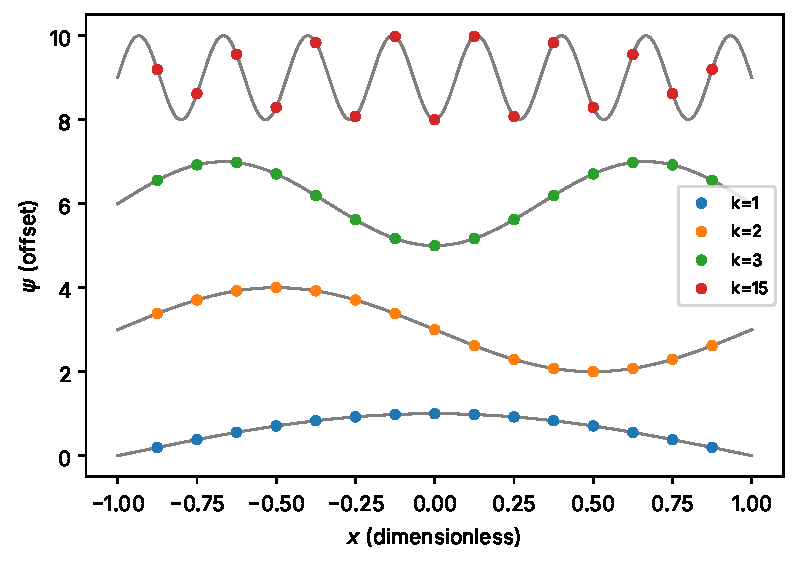
\includegraphics[width=0.85\linewidth]{figs/finite-differences_states.pdf}
\caption{Grid eigenvectors of the box $[-1,1]$ with $N=15$, rescaled so that $\sum_j\psi_j^2h=1$ (dots), against the continuum eigenfunctions $\sin(k\pi(x+L)/2L)/\sqrt L$ (curves), for $k=1,2,3$ and $k=N=15$; curves are offset vertically for clarity ($x$ dimensionless). For the box the grid vectors are exact samples. The $k=15$ vector is the nearly zigzag mode with about two points per wavelength, whose energy the grid underestimates most.}
\label{fig:finite-differences-states}
\end{figure}

\begin{checkpoint}
\texttt{eigh\_tridiagonal} returns an eigenvector with $\sum_ju_j^2=1$ on a grid with $h=0.01$. By what factor must you multiply it to obtain a wavefunction normalized as $\int\psi^2\,\dd x=1$?
\end{checkpoint}
\checkanswer{By $1/\sqrt h=10$, Eq.~\eqref{eq:finite-differences-rescale}.}

\begin{keyideas}
\item With Dirichlet walls, the trapezoid rule makes the grid normalization $\sum_j\psi_j^2h=1$, Eq.~\eqref{eq:finite-differences-norm}.
\item Solvers return unit vectors; divide by $\sqrt h$ to get wavefunctions. Signs are arbitrary.
\item Expectation values of $f(x)$ are $\sum_ju_j^2f(x_j)$; computed this way, $A_{nk}$ is the exact derivative of the grid eigenvalue, Eq.~\eqref{eq:finite-differences-Ank}.
\end{keyideas}

%==========================================================
\section{Correcting the targets instead of the operator}\label{sec:finite-differences-targets}

\subsection{Three ways to deal with grid bias}

Suppose you want to fit a potential so that its levels match a list of target numbers $t_n$ (in the paper, the zeros). A fit needs many eigensolves: every iteration solves for the levels and eigenvectors of the current potential, and an iteration may try several candidate steps (Chapter~\ref{ch:fitting}). You have three options for the grid bias.
\begin{enumerate}
\item \textbf{A very fine grid every time.} Accurate but expensive, as the brute-force Sample Problem showed.
\item \textbf{Richardson every time.} Two fine eigensolves per trial step instead of one working-grid solve.
\item \textbf{Correct the targets once.} Compute the bias for the \emph{unperturbed} potential once, before fitting, and move the targets by that amount. Then fit on a cheap working grid.
\end{enumerate}
The paper uses option 3. Let us define it precisely.

\subsection{Definitions}

Let $V$ be the smooth (unperturbed) potential. Compute its levels three times: on the working grid, giving $E_n^{g}[\mathrm{smooth}]$, and on two finer grids related by (nearly) exact halving (see \cref{sec:finite-differences-paper} and Problem~11 for the paper's pairs), combined by \eqref{eq:finite-differences-richardson} into $E_n^{\rm Rich}[\mathrm{smooth}]$, an estimate of the true continuum levels with only $\order(h^4)$ error. Define the \emph{grid bias}
\begin{equation}
\Delta_n=E_n^{g}[\mathrm{smooth}]-E_n^{\rm Rich}[\mathrm{smooth}]
\label{eq:finite-differences-Delta}
\end{equation}
and the \emph{bias-corrected targets}
\begin{equation}
\tilde t_n=t_n+\Delta_n.
\label{eq:finite-differences-ttilde}
\end{equation}
Since grid levels sit below the true ones (exactly for the box, \cref{sec:finite-differences-box}, and to leading order by the heuristic estimate of \cref{sec:finite-differences-bias} for smooth potentials), $\Delta_n$ is negative in practice and the corrected targets are lowered to where the working grid would place a level that is truly at $t_n$. The fit then compares working-grid eigenvalues $E_n[\mathrm{fit}]$ with $\tilde t_n$.

\subsection{The approximation being made}

Option 3 assumes that the grid bias of the \emph{fitted} potential equals that of the smooth potential, $E_n^{g}[\mathrm{fit}]-E_n^{\rm true}[\mathrm{fit}]\approx\Delta_n$. This is an approximation, and we should say when it holds.
\begin{itemize}
\item \textbf{Exactly true for a constant shift.} If $\delta V=c$ everywhere, the grid matrix changes by $c$ times the identity, so every grid eigenvalue shifts by exactly $c$; the continuum levels and the Richardson estimate also shift by exactly $c$. The difference $\Delta_n$ is unchanged.
\item \textbf{Approximately true for a small varying correction.} By \eqref{eq:finite-differences-bias-estimate} the bias depends on $\langle(E_n-V)^2\rangle$. Adding $\delta V$ changes $E_n-V$ to $E_n+\delta E_n-V-\delta V$. Problem~29 shows the bias then changes by approximately $-\tfrac{h^2}{6}\langle(E_n-V)(\delta E_n-\delta V)\rangle$, which is a small fraction of $\Delta_n$ as long as $\delta V-\delta E_n$ is small compared with the local kinetic energy $E_n-V$ over the region the level occupies.
\end{itemize}
The neglected piece is therefore the change of a correction that is itself of order two mean spacings, multiplied by a ratio like $2\abs{\delta V-\delta E_n}/(E_n-V)$ (Problem~29). As an order-of-magnitude estimate: if $\delta V-\delta E_n$ is $3\%$ of the local kinetic energy, the change is about $2\times0.03\times2=0.12$ spacings, roughly a tenth of a spacing; it is smaller where $\delta V$ oscillates and its effect averages out over the state. Keep in mind that this is an estimate built on the heuristic \eqref{eq:finite-differences-bias-estimate}.

\subsection{Why the correction leaks nothing: the identity of the paper's Eq.~(3)}

Here is a worry a careful referee raises. In an out-of-sample test, the fit sees only training zeros, and its predictions are scored on held-out zeros. But the corrected targets $\tilde t_n$ exist for \emph{every} index $n$, including the held-out ones. Could the correction smuggle information about the held-out zeros into the score?

Write the residual of the fitted level against the corrected target and substitute \eqref{eq:finite-differences-ttilde}:
\begin{align}
\tilde t_n-E_n[\mathrm{fit}]&=(t_n+\Delta_n)-E_n[\mathrm{fit}]\qquad\text{(definition of }\tilde t_n\text{)}\nonumber\\
&=t_n-E_n[\mathrm{fit}]+\Delta_n\qquad\text{(reorder)}\nonumber\\
&=t_n-\big(E_n[\mathrm{fit}]-\Delta_n\big).\qquad\text{(factor the minus sign)}
\label{eq:finite-differences-leakage}
\end{align}
This is the paper's Eq.~(3). Read the two ends of the chain as two different procedures:
\begin{itemize}
\item \emph{Left side:} compare the fitted level with the corrected target.
\item \emph{Right side:} first correct the \emph{prediction}, replacing $E_n[\mathrm{fit}]$ by $E_n[\mathrm{fit}]-\Delta_n$, then compare with the raw zero $t_n$.
\end{itemize}
They are the same number for every $n$, so every rms and every correlation computed from them is identical. Now ask what $\Delta_n$ is made of. By \eqref{eq:finite-differences-Delta} it is built only from eigenvalues of the \emph{unperturbed} potential on three grids. No zero, training or held-out, enters it. So the correction is a fixed, data-independent adjustment of the model's output, of the same kind as choosing a more accurate solver. Nothing about the held-out $t_n$ reaches the fit or the prediction except through the final comparison, where it must enter.

There is a second illuminating rewriting. The paper measures fluctuations relative to the unperturbed levels. The ``true fluctuation'' of level $n$ is then
\begin{align*}
\tilde t_n-E_n^{g}[\mathrm{smooth}]&=t_n+\big(E_n^{g}[\mathrm{smooth}]-E_n^{\rm Rich}[\mathrm{smooth}]\big)-E_n^{g}[\mathrm{smooth}]\\
&=t_n-E_n^{\rm Rich}[\mathrm{smooth}].
\end{align*}
The working-grid levels cancel, and what remains is the raw zero minus the continuum-accurate level of the smooth potential. That is exactly the quantity a physicist would want, freed of any grid artifact.

\begin{sample}{The leakage identity with numbers}
Take the paper's $t_{500}=811.1843588$ (Appendix~A, key anchors). Suppose, purely for illustration (these are not the paper's values), that $\Delta_{500}=-2.50$ and a fitted potential has $E_{500}[\mathrm{fit}]=808.50$. Compute the residual both ways.

\textbf{Step 1: Corrected target.} $\tilde t_{500}=811.1843588-2.50=808.6843588$.

\textbf{Step 2: Left side of \eqref{eq:finite-differences-leakage}.} $\tilde t_{500}-E_{500}[\mathrm{fit}]=808.6843588-808.50=0.1843588$.

\textbf{Step 3: Right side.} Corrected prediction $E_{500}[\mathrm{fit}]-\Delta_{500}=808.50+2.50=811.00$; residual $811.1843588-811.00=0.1843588$.

\begin{equation*}
\boxed{\text{Both procedures give the residual }0.1843588.}
\end{equation*}
\end{sample}

\begin{checkpoint}
Does the grid bias $\Delta_n$ depend on the value of any Riemann zero?
\end{checkpoint}
\checkanswer{No. By Eq.~\eqref{eq:finite-differences-Delta} it is a difference of eigenvalues of the unperturbed potential computed on different grids; no zero enters.}

\begin{pitfall}
``No leakage'' is a statement about \emph{information}, not about accuracy. The identity \eqref{eq:finite-differences-leakage} guarantees that the correction cannot help a model cheat. It does not guarantee that the correction is accurate for the fitted potential; that is the separate approximation discussed above, which affects all models and the null in the same way.
\end{pitfall}

\begin{keyideas}
\item The paper computes $\Delta_n=E^g_n[\mathrm{smooth}]-E^{\rm Rich}_n[\mathrm{smooth}]$ once and fits against $\tilde t_n=t_n+\Delta_n$ on a cheap working grid.
\item This assumes the fitted potential has nearly the same grid bias as the smooth one: exact for constant shifts, approximate otherwise.
\item $\tilde t_n-E_n[\mathrm{fit}]=t_n-(E_n[\mathrm{fit}]-\Delta_n)$, Eq.~\eqref{eq:finite-differences-leakage}: scoring against corrected targets equals correcting the prediction by a zero-free quantity. No held-out information leaks.
\end{keyideas}

%==========================================================
\section{Paper connection}\label{sec:finite-differences-paper}

Everything in this chapter was built to read the paper's ``forward solver''. Here it is, statement by statement.

\paragraph{The solver (Sec.~II~B, App.~A steps 3--4).} The paper works in units $\hbar=2m=1$ with $H=-\dd^2/\dd x^2+V(x)$, $V$ even. It uses ``second-order finite differences on $N$ uniform interior points (Dirichlet walls)'', which ``give a symmetric tridiagonal matrix; eigenpairs from LAPACK''. That is \cref{sec:finite-differences-grid} exactly: Appendix~A step 4 records the matrix as ``tridiagonal $\mathrm{diag}=2/dx^2+V$, off $=-1/dx^2$'' (the paper's $dx$ is our $h$) and the solver as \texttt{eigh\_tridiagonal}, the routine used in our listings. Step 3 records the grids: interior-point uniform on $(-L,L)$, scale~1 with $L=44.8827$ and working grid $N=6000$, scale~2 with $L=59.9572$ and $N=8000$. With $h=2L/(N+1)$ both scales have nearly the same spacing, $0.0149585$ and $0.0149874$ (Problem~1). The paper evaluates only the eigenvalues it needs: step 4 lists ranges $[0,900]$ for the scale-1 Hermitian work, $[0,1000]$ for the tensors of Sec.~II~E (652 states) and $[0,1500]$ at scale~2 (1079 states).

\paragraph{The potential on the grid (Sec.~II~B, App.~A step 3).} The Wu--Sprung potential is given implicitly by $x(V)$, Eq.~(2), which Chapter~\ref{ch:wu-sprung} derives. The paper inverts it ``by Brent inversion of Eq.~(2) on a dense reference grid, cubic-spline interpolated''. Richardson needs a smooth potential (condition 3 of \cref{sec:finite-differences-richardson}), so it is reassuring to check the bottom of the well. Put $V=V_0+\eta^2$ with $\eta=\sqrt{V-V_0}\ge0$ (a new symbol, unrelated to machine epsilon $\epsilon$ and to the perturbation parameter $\varepsilon$ of Eq.~\eqref{eq:finite-differences-hf}). First rationalize the argument of the second logarithm by multiplying numerator and denominator by $\sqrt V+\eta$:
\begin{equation*}
\frac{\sqrt V+\eta}{\sqrt V-\eta}=\frac{(\sqrt V+\eta)^2}{V-\eta^2}=\frac{(\sqrt V+\eta)^2}{V_0},
\end{equation*}
so Eq.~(2) reads
\begin{equation*}
x=\frac1\pi\left[\eta\log\frac{V_0}{2\pi e^2}+2\sqrt{V_0+\eta^2}\,\log\frac{\sqrt{V_0+\eta^2}+\eta}{\sqrt{V_0}}\right].
\end{equation*}
Now let $\eta$ be small. Then $\sqrt{V_0+\eta^2}\approx\sqrt{V_0}$, and with $\log(1+u)\approx u$ for small $u$, $\log\big[(\sqrt{V_0}+\eta)/\sqrt{V_0}\big]=\log(1+\eta/\sqrt{V_0})\approx\eta/\sqrt{V_0}$, so
\begin{equation*}
x\approx\frac1\pi\left[\eta\log\frac{V_0}{2\pi e^2}+2\eta\right]=\frac{\eta}{\pi}\log\frac{V_0}{2\pi}\qquad\text{(since }\log e^2=2\text{)}.
\end{equation*}
Solving for $\eta^2=V-V_0$, $V\approx V_0+\big(\pi/\log(V_0/2\pi)\big)^2x^2\approx V_0+51.3\,x^2$. This leading-order parabola does not by itself exclude higher terms such as $\abs{x}^3$, which would be a hidden kink. To exclude them, read the formula for $x$ as a function of $\eta$ allowed to take either sign. The factor $\sqrt{V_0+\eta^2}$ is even in $\eta$. The logarithm is odd in $\eta$, because $(\sqrt{V_0+\eta^2}-\eta)(\sqrt{V_0+\eta^2}+\eta)=V_0$ gives $\log\big[(\sqrt{V_0+\eta^2}-\eta)/\sqrt{V_0}\big]=-\log\big[(\sqrt{V_0+\eta^2}+\eta)/\sqrt{V_0}\big]$. The first term is odd as well. So $x(\eta)$ is an odd smooth function with nonzero slope $\log(V_0/2\pi)/\pi$ at $\eta=0$ (here $V_0/2\pi=1.550$, whose logarithm is positive). A smooth function with nonzero slope has a smooth inverse (first-year calculus), so $\eta$ is a smooth odd function of $x$, and $V=V_0+\eta^2$ is a smooth even function of $x$: no kink at $x=0$. The code below reproduces the paper's construction with a spline, and evaluating \texttt{x\_of\_V(1000.0)} returns $44.883$, the paper's scale-1 half-width $L$.

\begin{pycode}
import numpy as np
from scipy.interpolate import CubicSpline
V0 = 3.10073 * np.pi

def x_of_V(V):                      # paper Eq. (2); note (r+s)/(r-s) = (r+s)^2/V0
    s, r = np.sqrt(V - V0), np.sqrt(V)
    return (s * np.log(V0 / (2*np.pi*np.e**2))
            + r * np.log((r + s)**2 / V0)) / np.pi

u = np.linspace(0, np.sqrt(1100 - V0), 40001)   # V = V0 + u^2, dense near bottom
spline = CubicSpline(x_of_V(V0 + u**2), u)
V_of_x = lambda x: V0 + spline(np.abs(x))**2     # even in x
L = x_of_V(1000.0)                               # about 44.883
\end{pycode}

\paragraph{Correcting the targets (Sec.~II~B, App.~A step 5).} The paper states that ``discretization bias is removed from the \emph{targets} rather than the operator'': all fitting runs on the working grid against $\tilde t_n=t_n+(E^{\rm grid}_n[\mathrm{smooth}]-E^{\rm Rich}_n[\mathrm{smooth}])$. That is \eqref{eq:finite-differences-Delta}--\eqref{eq:finite-differences-ttilde}. The Richardson pairs are $12000/24000$ (scale~1) and $16000/32000$ (scale~2). Because $h=2L/(N+1)$, doubling $N$ from $12000$ to $24000$ halves $h$ only approximately ($r=24001/12001$); Problem~11 shows the leftover $h^2$ error is below $3\times10^{-5}$ of the coarse grid's, utterly negligible.

\begin{pitfall}
The paper writes the extrapolation compactly as ``$E^{\rm Rich}=(4E_{2h}-E_h)/3$ \ldots\ over grid doubling''. The derivation of \cref{sec:finite-differences-richardson} shows that the weight 4 must go to the \emph{finer} grid. We therefore read the paper's subscripts (this is our interpretation; the paper does not spell it out) as labels for the grid with twice as many points (the second member of each listed pair, $24000$ or $32000$), not as a spacing of $2h$. In terms of spacings the formula is $(4E_{h/2}-E_h)/3$, Eq.~\eqref{eq:finite-differences-richardson}. If you reconstruct the pipeline, give the weight 4 to the finer grid; Problem~31 shows that the opposite assignment is worse than no extrapolation at all.
\end{pitfall}

\paragraph{How good is the smooth potential after correction (Sec.~II~B).} The paper reports that ``the residual of $E^{\rm Rich}$ against the smooth zeros is $0.005$ spacings mean, $0.063$ max (worst at low $n$, the known semiclassical weakness of the construction)''. Read this carefully: once the grid bias is removed, what remains is not a grid error but a property of the Wu--Sprung potential itself. That potential is built from a semiclassical approximation (Chapter~\ref{ch:wkb}) that is least accurate for the lowest levels (Chapter~\ref{ch:wu-sprung}). Richardson cannot and should not remove it. \Cref{fig:finite-differences-wsbias} shows both quantities computed with the spline construction above.

\begin{figure}[htbp]\centering
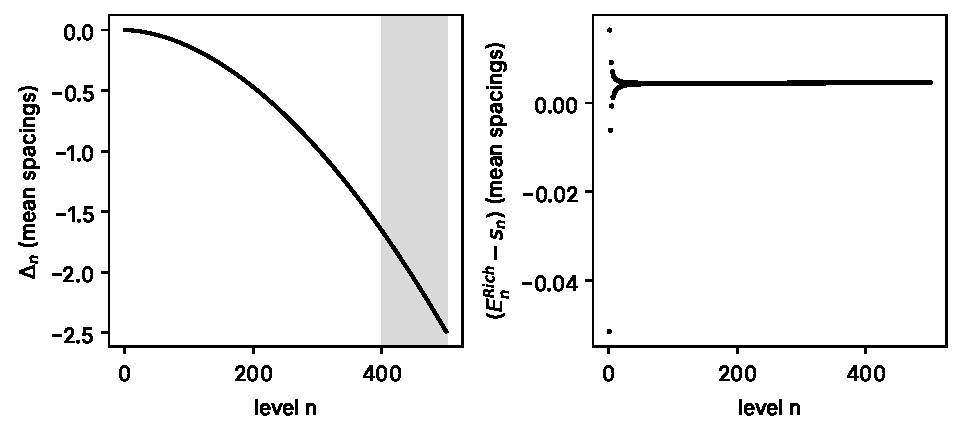
\includegraphics[width=0.85\linewidth]{figs/finite-differences_wsbias.pdf}
\caption{The Wu--Sprung potential at scale 1 ($L=x(1000)$, units $\hbar=2m=1$), computed with the spline construction of this section. Left: grid bias $\Delta_n=E^g_n-E^{\rm Rich}_n$ on the working grid $N=6000$, with $E^{\rm Rich}$ from $N=12000$ and $24000$, in units of the local mean spacing $\mathrm{gap}_n=2\pi/\log(s_n/2\pi)$; the paper reports that this bias reaches about two mean spacings at levels 401--500 (Sec.~II~C). Right: $(E^{\rm Rich}_n-s_n)/\mathrm{gap}_n$, the residual of the extrapolated levels against the smooth zeros; the paper reports mean $0.005$ and maximum $0.063$ spacings, largest at low $n$ (Sec.~II~B).}
\label{fig:finite-differences-wsbias}
\end{figure}

\paragraph{No leakage (Sec.~II~C, Eq.~(3)).} The paragraph ``No leakage through the bias correction'' is the identity \eqref{eq:finite-differences-leakage}: ``scoring the fit against $\tilde t_n$ is algebraically identical to correcting the \emph{prediction} by the fit-independent quantity $\Delta_n$ and scoring against the raw zeros''; $\Delta_n$ ``is built solely from eigenvalues of the \emph{unperturbed} potential on two grids; no zero, in-sample or held-out, enters it''. (The paper's ``two grids'' refers to the Richardson pair. The full $\Delta_n$ of Eq.~\eqref{eq:finite-differences-Delta} uses three grids: the working grid supplies $E^g_n$ and the pair supplies $E^{\rm Rich}_n$. None of the three involves a zero.) The paper also states why the correction cannot be skipped: finite-difference dispersion ``at levels 401--500 on the working grid reaches two mean spacings and would otherwise dominate both the null and every model identically''. Appendix~A (step 20, revision computations) adds an empirical counterpart for the sinusoidal controls: ``Overwriting held-out data with noise before fitting leaves all fitted coefficients bit-identical''. The sentence follows step 20, which describes the sinusoidal controls, and we read it as referring to them; the paper does not say explicitly whether the operator fits were tested in the same way. For the operator fits the guarantee we can verify ourselves is the algebraic identity \eqref{eq:finite-differences-leakage} together with the zero-free construction of $\Delta_n$.

\paragraph{The raw-zero null 2.09 (App.~A, key anchors).} The null model of Sec.~II~C is the unperturbed potential itself. Scored against corrected targets, its error on zeros 401--500 is $0.2631$ mean spacings (key anchors; $0.263$ in the tables). By the rewriting in \cref{sec:finite-differences-targets}, this is the rms of $t_n-E_n^{\rm Rich}[\mathrm{smooth}]$, the genuine fluctuation of the zeros about the smooth levels. Scored instead against the \emph{raw} zeros on the uncorrected working grid, the same null gives $2.09$. That number is dominated by the grid bias of about two spacings reported by the paper (Sec.~II~C) and plotted in \cref{fig:finite-differences-wsbias}; the real fluctuations of size $0.26$ are buried underneath it (Problem~14). This is also why the paper's two nulls can coincide numerically (Sec.~II~C): after correction, $E_n^{\rm Rich}[\mathrm{smooth}]$ agrees with the smooth zeros $s_n$ to $0.005$ spacings on average, so ``unperturbed levels'' and ``smooth zeros'' are, as predictions, nearly the same.

\paragraph{Normalization and the sensitivity matrix (Sec.~II~C, App.~A steps 6, 9).} The fit uses $A_{nk}=\int\abs{\psi_n}^2\cos(k\pi x/L)\,\dd x$, and Appendix~A step 9 records ``$\psi$ normalized $\sum\psi^2dx=1$'', Eq.~\eqref{eq:finite-differences-norm}. By \eqref{eq:finite-differences-Ank}, the grid sum is the exact derivative of the grid eigenvalue with respect to $c_k$, which is what an iterated linearization needs (Chapter~\ref{ch:fitting}).

\paragraph{Exact checks on a coarser grid (App.~A step 11).} The non-Hermitian checks of Sec.~V diagonalize the complex matrix of $H+iA$ densely on $N=2500$, a coarser common grid; dense complex eigensolves cost far more than tridiagonal ones (Chapters~\ref{ch:eigen} and \ref{ch:non-hermitian}). Those checks compare two calculations on the same grid, so the grid bias is common to both.

\paragraph{The interpolation split (Sec.~III, Fig.~4).} When the paper says ``$x$ and $V$ are in the units $\hbar=2m=1$ of Sec.~II~B'', and reports a fitted correction with maximum $\abs{\delta V}=199$ where the smooth potential is about 500, it is describing a potential on exactly the grid of this chapter. A correction of that size is a large fraction of the local kinetic energy, the regime where the target-correction approximation of \cref{sec:finite-differences-targets} is least accurate. The paper does not quantify how much $\Delta_n$ changes there. By the estimate of Problem~29 the change could be a sizeable fraction of $\Delta_n$ itself, which at levels 201--300 is presumably below its size of about two spacings at 401--500 (the bias grows with energy). That would still be smaller than the $2.64$-spacing gap error the paper reports, but we have not verified it numerically: read this as a plausibility argument, not a result.

%==========================================================
\section{Summary}\label{sec:finite-differences-summary}

\begin{itemize}
\item The central second difference satisfies $D_h^2f=f''+\tfrac{h^2}{12}f''''+\tfrac{h^4}{360}f^{(6)}+\cdots$, Eq.~\eqref{eq:finite-differences-second-difference}: second-order accurate, even powers of $h$ only. Roundoff adds an error of order $\epsilon/h^2$, Eq.~\eqref{eq:finite-differences-roundoff}.
\item On $N$ interior points with $h=2L/(N+1)$ and Dirichlet walls, $-\psi''+V\psi=E\psi$ becomes $\mathsf H\bm\psi=E\bm\psi$ with the symmetric tridiagonal $\mathsf H$ of Eq.~\eqref{eq:finite-differences-matrix}: diagonal $2/h^2+V_j$, off-diagonals $-1/h^2$.
\item The discrete box is exact: $E_k^{(h)}=(4/h^2)\sin^2(k\pi h/4L)$, Eq.~\eqref{eq:finite-differences-box-exact}, eigenvectors are sampled continuum sines, and $E_k^{(h)}=E_k-h^2E_k^2/12+h^4E_k^3/360-\cdots$, Eq.~\eqref{eq:finite-differences-box-expansion}.
\item Numerical dispersion: the grid gives a wave of wavenumber $q$ the kinetic energy $(4/h^2)\sin^2(qh/2)$, Eq.~\eqref{eq:finite-differences-dispersion}; accuracy is governed by points per wavelength, \cref{tab:finite-differences-ppw}.
\item For a symmetric matrix, $\dd E/\dd\varepsilon=\mathbf u^\top\mathsf W\mathbf u$, Eq.~\eqref{eq:finite-differences-hf}; heuristically the grid bias of level $n$ is $-\tfrac{h^2}{12}\langle(E_n-V)^2\rangle$, Eq.~\eqref{eq:finite-differences-bias-estimate}.
\item Richardson: $(4E(h/2)-E(h))/3=E+\order(h^4)$, Eq.~\eqref{eq:finite-differences-richardson}; general ratio, Eq.~\eqref{eq:finite-differences-richardson-r}; box residual $\approx-h^4E^3/1440$, Eq.~\eqref{eq:finite-differences-rich-box}.
\item Grid normalization $\sum_j\psi_j^2h=1$, Eq.~\eqref{eq:finite-differences-norm}; solver unit vectors are divided by $\sqrt h$, Eq.~\eqref{eq:finite-differences-rescale}; $A_{nk}$ computed by grid sums is the exact grid derivative, Eq.~\eqref{eq:finite-differences-Ank}.
\item The paper corrects targets: $\tilde t_n=t_n+\Delta_n$ with $\Delta_n=E^g_n-E^{\rm Rich}_n$ of the smooth potential, Eqs.~\eqref{eq:finite-differences-Delta}--\eqref{eq:finite-differences-ttilde}; the leakage identity $\tilde t_n-E_n[\mathrm{fit}]=t_n-(E_n[\mathrm{fit}]-\Delta_n)$, Eq.~\eqref{eq:finite-differences-leakage}, is the paper's Eq.~(3).
\item Without the correction, the grid bias (about two mean spacings at levels 401--500) swamps the fluctuations: the paper's raw-zero null is $2.09$ against $0.263$ corrected.
\end{itemize}

%==========================================================
\section{Problems}\label{sec:finite-differences-problems}

\begin{problemlist}
\prob{1}{Compute the grid spacing $h=2L/(N+1)$ for the paper's two working grids: scale~1 with $L=44.883$, $N=6000$, and scale~2 with $L=59.957$, $N=8000$. What do you notice?}

\prob{1}{How many nonzero entries does the $N\times N$ matrix \eqref{eq:finite-differences-matrix} have? For $N=6000$, what fraction of all $N^2$ entries is that?}

\prob{1}{Use the forward difference \eqref{eq:finite-differences-forward} with $h=0.01$ to estimate the derivative of $e^x$ at $x=0$. Compare the error with the prediction $\tfrac h2f''$.}

\prob{1}{By what factor does the error of a computed box level fall when $h$ is halved (a) for the raw grid value, (b) for the Richardson combination? Assume the asymptotic regime.}

\prob{2}{Apply Richardson's idea to the second difference itself: show that $\tfrac13[4D_h^2f-D_{2h}^2f]$ equals $\big[-f(x+2h)+16f(x+h)-30f(x)+16f(x-h)-f(x-2h)\big]/(12h^2)$, and explain why this five-point formula has an error of order $h^4$.}

\prob{2}{For the discrete box, show that $k=N+1$ in $\psi_j=\sin(jk\pi/(N+1))$ gives the zero vector, and that $k$ and $2(N+1)-k$ give the same vector up to sign. Conclude that there are only $N$ distinct eigenvectors.}

\prob{2}{Take the box $[-1,1]$ with only $N=1$ interior point. Find the single grid eigenvalue and its error. Then combine it with the $N=3$ ground state ($2.343146$) by Richardson. What is the error now?}

\prob{2}{For RE3 ($L=44.883$, $N=6000$), use the leading term of \eqref{eq:finite-differences-box-expansion} to estimate the error of box level $k=250$, in energy units and in units of the box level spacing $(2k+1)(\pi/2L)^2$.}

\prob{2}{Prove that $\sum_{j=1}^{N}\sin^2\!\big(jk\pi/(N+1)\big)=(N+1)/2$ for $1\le k\le N$. (Hint: write $\sin^2=\tfrac12(1-\cos)$ and sum the cosines as the real part of a geometric series of $z=e^{2\pi ik/(N+1)}$.) Deduce that the normalized discrete box eigenvector is $\psi_j=\sin(jk\pi/(N+1))/\sqrt L$, matching the continuum normalization.}

\prob{2}{Derive the Gaussian moments used in the harmonic-oscillator Sample Problem by integration by parts, and then estimate the grid bias of the first excited state $\psi_1\propto xe^{-x^2/2}$, $E_1=3$, for $h=0.1$.}

\prob{2}{The paper's Richardson pair at scale~1 is $N=12000$ and $N=24000$ with $L$ fixed. Find the exact refinement ratio $r$ of the spacings, and use \eqref{eq:finite-differences-richardson-r} to show that applying the $r=2$ formula leaves a fraction $(4/r^2-1)/3$ of the coarse grid's $h^2$ error uncancelled. Evaluate it.}

\prob{3}{Using numpy and \texttt{eigh\_tridiagonal}, compute the first 21 levels of $H=-\dd^2/\dd x^2+x^2$ on $[-10,10]$ with $h=0.1$. You may use the known result $\langle x^4\rangle_n=\tfrac34(2n^2+2n+1)$ and $\langle x^2\rangle_n=n+\tfrac12$ for this oscillator. Show that \eqref{eq:finite-differences-bias-estimate} predicts a bias $-\tfrac{h^2}{32}(E_n^2+1)$ with $E_n=2n+1$, and compare with your numbers. Why is it smaller than the box formula $-h^2E^2/12$ at the same energy?}

\prob{2}{(Paper.) A student argues: ``The corrected targets $\tilde t_n$ are defined for held-out $n$, so the out-of-sample score in the paper is contaminated.'' Using Eq.~(3) of the paper (our Eq.~\eqref{eq:finite-differences-leakage}) and the definition of $\Delta_n$, explain precisely why the student is wrong. Would the conclusion change if $\Delta_n$ were computed from the fitted potential rather than the smooth one?}

\prob{2}{(Paper.) The paper's raw-zero null on 401--500 is $2.09$ spacings, the corrected null $0.263$. Model the uncorrected residual as a constant bias $b$ plus a fluctuation with rms $0.263$ and zero mean. What value of $b$ reproduces $2.09$? Compare with the paper's statement that the dispersion ``reaches two mean spacings''. What does the model leave out?}

\prob{2}{Using \texttt{qmnt.fd\_levels} with $V=0$, $L=44.883$, $N=6000$, compute level 500 and compare with \eqref{eq:finite-differences-box-exact} and with the continuum value.}

\prob{2}{(Paper.) Using the spline construction of \cref{sec:finite-differences-paper} or \texttt{qmnt}, compute the Wu--Sprung levels on $N=6000$, $12000$, $24000$ at scale~1, form $\Delta_n$, and express it in units of $\mathrm{gap}_n$ (\texttt{qmnt.mean\_gap}). Compare the size on 401--500 with the paper's ``two mean spacings''.}

\prob{3}{Show that every eigenvalue of the discrete box lies strictly between $0$ and $4/h^2$. Find the largest eigenvalue for $L=44.883$, $N=6000$. What does its eigenvector look like, and is it a good approximation of any physical level?}

\prob{2}{How many continuum box levels with $L=44.883$ lie below $E=1000$? How many grid levels with $N=6000$? Explain the direction of the difference. (Compare with the paper's count of 652 Wu--Sprung states below $E=1000$, App.~A step 4.)}

\prob{1}{Check the leakage identity numerically with $t_n=50.000$, $\Delta_n=-0.30$, $E_n[\mathrm{fit}]=49.65$.}

\prob{2}{Show that if $V$ is even and the grid symmetric, the matrix $\mathsf H$ commutes with the reversal $j\to N+1-j$, and hence that every eigenvector is either symmetric or antisymmetric under reversal. Relate this to the parity of states in Chapter~\ref{ch:bound-states}.}

\prob{2}{Show that the central first difference $[f(x+h)-f(x-h)]/(2h)$ equals $f'+\tfrac{h^2}{6}f'''+\order(h^4)$, and test it on $\sin x$ at $x=1$ with $h=0.1$.}

\prob{3}{Starting from $\sin^2y=y^2-y^4/3+2y^6/45-y^8/315+\cdots$, derive the $h^4$ and $h^6$ terms of $E_k^{(h)}$ for the box, and show that the Richardson combination leaves $-h^4E^3/1440+E^4h^6/64512+\cdots$.}

\prob{2}{(Paper.) Apply the box estimate $h^2E^2/12$ with the paper's scale-1 spacing to $E=t_{500}=811.18$, and express it in units of the mean spacing $2\pi/\log(t/2\pi)$ at that height. Compare with the paper's ``two mean spacings''. Using \eqref{eq:finite-differences-bias-estimate}, explain the difference.}

\prob{3}{Write your own solver (no \texttt{qmnt.fit\_potential}) for the Wu--Sprung levels at scale~1 and compute $(E^{\rm Rich}_n-s_n)/\mathrm{gap}_n$ for $n=1,\dots,500$. Compare the mean and maximum with the paper's $0.005$ and $0.063$. Where is the maximum, and why there?}

\prob{2}{For the box $[-1,1]$, compute the ground-state error on grids with $N+1=4,8,16,32$ and the ratios of successive errors. What value should the ratios approach, and how does this test the ``asymptotic regime'' condition of Richardson extrapolation?}

\prob{2}{(Paper.) Appendix~A step 4 asks \texttt{eigh\_tridiagonal} only for eigenvalues in $[0,900]$ at scale~1, out of $N=6000$. Give two reasons not to compute all of them.}

\prob{1}{Why does the paper fit on a working grid of $N=6000$ rather than directly on the $N=24000$ grid used for Richardson?}

\prob{2}{Show that adding a constant $c$ to the potential leaves $\Delta_n$ exactly unchanged, by examining the grid matrix and the Richardson combination.}

\prob{3}{Using \eqref{eq:finite-differences-bias-estimate}, and neglecting the change of $\psi_n$, show that a correction $\delta V$ that shifts level $n$ by $\delta E_n$ changes the grid bias by approximately $-\tfrac{h^2}{6}\langle(E_n-V)(\delta E_n-\delta V)\rangle$. State a condition under which the paper's target correction remains accurate for a fitted potential.}

\prob{2}{Using numpy only (\texttt{np.diag}), build the $5\times5$ matrix for the box $[-1,1]$, compute its eigenvalues with \texttt{np.linalg.eigvalsh}, and check them against \eqref{eq:finite-differences-box-exact}.}

\prob{2}{(Paper.) Suppose a reconstruction used the weights the wrong way round, $(4E_{\rm coarse}-E_{\rm fine})/3$. Evaluate this for the box $[-1,1]$ with the $N=3$ and $N=7$ ground states, and compare with the correct Richardson value and with the raw values.}

\prob{2}{For the box $[-L,L]$, compute $A_{2,1}=\int\psi_2^2\cos(\pi x/L)\,\dd x$ and $A_{2,2}=\int\psi_2^2\cos(2\pi x/L)\,\dd x$, where $\psi_2=\sin(\pi x/L)/\sqrt L$. Verify them with a grid sum \eqref{eq:finite-differences-expect} for $L=1$, $N=99$.}
\end{problemlist}

%==========================================================
\section{Answers to selected problems}\label{sec:finite-differences-answers}
% DYK-BEGIN

% DYK-END

\textbf{1.} Scale~1: $h=89.766/6001=0.0149585$. Scale~2: $h=119.914/8001=0.0149874$. The two spacings agree to about $0.2\%$: the paper increased $N$ in proportion to $L$, so the grid resolution is essentially the same at both scales. (The scale-2 levels go higher, so their bias is still larger.)

\textbf{2.} $N$ diagonal entries plus $N-1$ on each off-diagonal: $3N-2$. For $N=6000$: $17998$ entries out of $3.6\times10^7$, a fraction $5.0\times10^{-4}$. This is why the matrix is passed to the solver as two diagonals.

\textbf{3.} $(e^{0.01}-1)/0.01=1.0050167$. The exact derivative is $1$, so the error is $0.0050167$; the prediction $\tfrac h2f''(0)=0.005$ accounts for it, the remainder being the $h^2f'''/6$ term.

\textbf{4.} (a) By 4, since the error is $\order(h^2)$. (b) By 16, since the Richardson error is $\order(h^4)$, Eq.~\eqref{eq:finite-differences-richardson}.

\textbf{5.} $D_{2h}^2f=[f(x+2h)-2f(x)+f(x-2h)]/(4h^2)$. Then
\begin{align*}
4D_h^2f-D_{2h}^2f&=\frac{16f(x+h)-32f(x)+16f(x-h)}{4h^2}-\frac{f(x+2h)-2f(x)+f(x-2h)}{4h^2}\\
&=\frac{-f(x+2h)+16f(x+h)-30f(x)+16f(x-h)-f(x-2h)}{4h^2},
\end{align*}
and dividing by 3 gives the stated formula. By \eqref{eq:finite-differences-second-difference}, $D_h^2f=f''+\tfrac{h^2}{12}f''''+\order(h^4)$ and $D_{2h}^2f=f''+\tfrac{4h^2}{12}f''''+\order(h^4)$, so $4D_h^2f-D_{2h}^2f=3f''+\order(h^4)$: the $h^2$ terms cancel exactly as in \cref{sec:finite-differences-richardson}.

\textbf{7.} $N=1$ gives $h=1$ and the $1\times1$ matrix $2/h^2=2$. The exact value is $\pi^2/4=2.467401$, so the error is $0.467$ ($18.9\%$; one interior point means four points per wavelength counting the walls, as in \cref{tab:finite-differences-ppw}). Richardson with $h=1$ and $h=0.5$: $(4\times2.343146-2)/3=2.457528$, error $0.00987$, almost fifty times smaller than the raw coarse error.

\textbf{9.} With $\sin^2a=\tfrac12(1-\cos2a)$,
\begin{equation*}
\sum_{j=1}^{N}\sin^2\frac{jk\pi}{N+1}=\frac N2-\frac12\sum_{j=1}^{N}\cos\frac{2jk\pi}{N+1}.
\end{equation*}
Let $z=e^{2\pi ik/(N+1)}$. For $1\le k\le N$, $z\ne1$ but $z^{N+1}=e^{2\pi ik}=1$, so the geometric series (Chapter~\ref{ch:series}) gives $\sum_{j=0}^{N}z^j=(1-z^{N+1})/(1-z)=0$. Removing the $j=0$ term, $\sum_{j=1}^{N}z^j=-1$; its real part is $\sum_{j=1}^N\cos(2jk\pi/(N+1))=-1$. Hence the sum is $N/2+1/2=(N+1)/2$. (Check: $N=3$, $k=1$: $0.5+1+0.5=2$.) For $\psi_j=A\sin(\cdots)$, \eqref{eq:finite-differences-norm} requires $A^2(N+1)h/2=1$, and $(N+1)h=2L$, so $A^2=1/L$: exactly the continuum normalization constant of the box.

\textbf{11.} $h_c/h_f=(24001)/(12001)=r=1.99992$. With $E_c=E+Ch_c^2$ and $E_f=E+Ch_c^2/r^2$, the $r=2$ formula gives $(4E_f-E_c)/3=E+Ch_c^2(4/r^2-1)/3$. Numerically $4/r^2=1.0000833$, so the uncancelled fraction is $2.78\times10^{-5}$ of the coarse ($N=12000$) grid's $h^2$ error. Since that error is of order a fraction of a mean spacing at these levels, the leftover is of order $10^{-5}$ spacings: negligible.

\textbf{13.} By Eq.~\eqref{eq:finite-differences-leakage}, scoring against $\tilde t_n$ is identical, number by number, to scoring the adjusted prediction $E_n[\mathrm{fit}]-\Delta_n$ against the raw zeros. The adjustment $\Delta_n$ is computed from eigenvalues of the smooth potential on three grids, before any fit, without any zero. So the held-out zeros enter only in the final comparison, which is what out-of-sample scoring means. If $\Delta_n$ were computed from the fitted potential instead, it would still contain no zero (the fitted potential depends only on training zeros), so there would still be no leakage; it would merely be a slightly more accurate, fit-dependent correction, at the cost of extra fine-grid eigensolves.

\textbf{15.} \texttt{qmnt.fd\_levels(np.zeros(6000), 44.883, k=500)[-1]} gives $304.46$, matching \eqref{eq:finite-differences-box-exact} (agreement to better than $10^{-8}$); the continuum value is $306.21$, so the grid is $1.74$ too low, $1.42$ box level spacings (RE3 Sample Problem).

\textbf{17.} The eigenvalues are $(4/h^2)\sin^2(k\pi/(2(N+1)))$ with $0<k\pi/(2(N+1))<\pi/2$ for $1\le k\le N$, so $0<\sin^2<1$ and $0<E^{(h)}_k<4/h^2$. The largest is $k=N$: $(4/h^2)\cos^2(\pi/(2(N+1)))$, which for $N=6000$ is $17876.5$ (the cosine factor differs from 1 by less than $10^{-7}$). Its eigenvector $\sin(jN\pi/(N+1))=(-1)^{j+1}\sin(j\pi/(N+1))$ alternates in sign from point to point, the zigzag mode of \cref{fig:finite-differences-states}. Its continuum partner would have energy $(N\pi/2L)^2\approx4/h^2\times(\pi/2)^2$, about $2.5$ times larger; it is not a usable approximation of any physical level. Only levels with $k\ll N$ are physical.

\textbf{19.} $\tilde t_n=50.000-0.30=49.70$, and $\tilde t_n-E_n[\mathrm{fit}]=0.05$. Corrected prediction $49.65+0.30=49.95$, and $t_n-49.95=0.05$. Same residual.

\textbf{21.} Subtract \eqref{eq:finite-differences-taylor-minus} from \eqref{eq:finite-differences-taylor-plus}: even powers cancel, odd powers double, $f(x+h)-f(x-h)=2hf'+\tfrac{h^3}{3}f'''+\order(h^5)$; divide by $2h$ to get $f'+\tfrac{h^2}{6}f'''+\order(h^4)$. For $\sin$ at $1$ with $h=0.1$: $[\sin1.1-\sin0.9]/0.2=\cos1\,\sin(0.1)/0.1=0.5394022$, against $\cos1=0.5403023$: error $-9.0005\times10^{-4}$, prediction $\tfrac{h^2}{6}(-\cos1)=-9.0050\times10^{-4}$.

\textbf{23.} $h^2=2.23757\times10^{-4}$, $E^2=811.18^2=6.580\times10^5$, so $h^2E^2/12=12.3$ energy units. The mean spacing near $t=811$ is $2\pi/\log(811.18/2\pi)=1.293$, so the box estimate is $9.5$ spacings, several times the paper's ``two mean spacings''. The box formula assumes all of $E$ is kinetic energy everywhere. In the Wu--Sprung well, Eq.~\eqref{eq:finite-differences-bias-estimate} averages $(E-V)^2$. In the Wu--Sprung well $V$ rises from $V_0\approx9.7$ to $E$ across the allowed region, so $E-V$ is well below $E$ over most of it and tends to zero at the turning points, where the state spends much of its time. Both effects make $\langle(E-V)^2\rangle$ much smaller than $E^2$.

\textbf{25.} With $E_1=\pi^2/4=2.4674011$: errors $0.12426$ ($N+1=4$), $0.031546$ ($8$), $0.0079170$ ($16$), $0.0019811$ ($32$). Ratios $3.94$, $3.98$, $4.00$, approaching $4=2^2$. Ratios close to 4 show the $h^2$ term dominates, so Richardson's cancellation is valid; a ratio far from 4 would warn that the grid is too coarse (or the potential not smooth).

\textbf{27.} Each fit iteration requires at least one eigensolve with eigenvectors for all fitted levels, and several trial steps (Chapter~\ref{ch:fitting}). The cost and memory of such a solve grow at least in proportion to $N$, so the $N=24000$ grid would make every one of these solves several times more expensive. The target correction delivers essentially the accuracy of the Richardson grids at the price of three eigensolves of the smooth potential, done once, while the fit itself runs on the cheap grid.

\textbf{29.} To first order in small quantities, $(E_n+\delta E_n-V-\delta V)^2=(E_n-V)^2+2(E_n-V)(\delta E_n-\delta V)+\cdots$. Inserting into \eqref{eq:finite-differences-bias-estimate} with $\psi_n$ held fixed, the bias changes by $-\tfrac{h^2}{12}\cdot2\langle(E_n-V)(\delta E_n-\delta V)\rangle=-\tfrac{h^2}{6}\langle(E_n-V)(\delta E_n-\delta V)\rangle$. Compared with the bias itself, $-\tfrac{h^2}{12}\langle(E_n-V)^2\rangle$, this is a relative change of order $2\abs{\delta E_n-\delta V}/(E_n-V)$. So the correction stays accurate when $\delta V$ departs from a constant by much less than the local kinetic energy $E_n-V$ over the region the level occupies. For a constant $\delta V$, $\delta E_n=\delta V$ and the change vanishes, consistent with Problem~28.

\textbf{31.} $(4\times2.343146-2.435855)/3=2.312243$, error $0.155$, worse than either raw value (errors $0.124$ and $0.032$), and far worse than the correct Richardson value $2.466758$ (error $6.4\times10^{-4}$). Putting the weight on the coarse grid amplifies the $h^2$ error instead of cancelling it.
